\chapter{突触连接的经验和细化} \label{chap:chap49}


人类的神经系统在出生时就具有功能:新生儿可以看、听、呼吸和吮吸。
然而,与其他物种相比,人类婴儿的能力还很初级。
角马幼崽在出生后几分钟内就能站立和奔跑,许多鸟类从蛋中孵化后不久就能飞翔。
相比之下,人类婴儿要到 2 个月大才能抬起头,要到 6 个月大才能把食物送到嘴里,如果没有父母的照顾,十年也活不下去。


是什么导致了我们的运动、知觉和认知能力的延迟成熟?
一个主要因素是第~\ref{chap:chap45}~章到第~\ref{chap:chap48}~章中讨论的神经系统的胚胎连通性只是存在于我们成人自身中的神经回路的“粗略草稿”。
胚胎回路通过感官刺激(我们的经验)得到完善。
这个由两部分组成的序列(基因决定的连通性,然后是依赖经验的重组)是哺乳动物神经发育的一个共同特征,但在人类中,第二阶段特别长。


乍一看,人类神经发育的这种延迟似乎是不正常的。
它确实付出了代价,但它也提供了一个优势。
因为我们的心智能力很大程度上是由经验塑造的,所以我们获得了使我们的神经系统适应我们个人身体和独特环境的能力。
有人认为,不仅仅是人类大脑的体积大,而且它依赖于经验的成熟使我们的心智能力优于其他物种。


神经系统对经验做出反应的可塑性贯穿一生。
然而,在发育的特定时期会出现对修饰高度敏感的时期,称为敏感期。
在某些情况下,通过在晚年提供适当的经验,无法轻易扭转早年受限时期的剥夺或非典型经历的不利影响。
这样的时期被称为关键时期。
正如我们将看到的,新发现正在模糊敏感时期和关键时期之间的区别,因此我们将使用术语“关键时期”来指代两者。


行为观察帮助我们了解关键时期。
印记是鸟类的一种学习形式,是在关键时期建立的终生行为的最引人注目的例证之一。
刚孵出后,鸟类就会对环境中一个突出的移动物体产生不可磨灭的依恋或印记,并跟随它四处走动。
这通常是它们的母亲,但也可能是靠近新生小鸡的实验者。 印记过程对于保护幼崽很重要。
尽管这种依恋可以迅速获得并持续存在,但印记只能在孵化后不久的关键时期发生:在某些物种中,只有几个小时。


在人类中,儿童获得感知周围世界、学习语言或建立社会关系的能力的方式很明显。
一个 5 岁的孩子可以快速、毫不费力地学习第二语言,而一个 15 岁的青少年可能会流利,但说话时可能带有口音,即使他活到 90 岁。
同样,在生命的最初 3 到 4 年内安装了人工耳蜗的聋儿通常可以很好地掌握和理解口语,而在以后的年龄中,无论是表达还是理解都可能永远不会正常。
这些关键时期表明,依赖于经验的神经发育集中在(尽管肯定不限于)出生后早期。


在本章的开头,我们将考察早期经验塑造一系列人类心理能力的证据,从我们理解所见事物的能力到我们参与适当社会互动的能力。
这些经验效应的神经基础已经在实验动物大脑的许多部分进行了分析,包括听觉、体感、运动和视觉系统。
在这里,我们将主要关注视觉系统,而不是调查多个系统,因为对该系统的研究提供了对经验如何塑造神经回路的特别丰富的理解。
我们将看到,需要经验来改进突触连接的模式,并在这些模式形成后稳定它们。
最后,我们将考虑最近的证据,表明许多系统中的关键时期没有以前想象的那么严格,在某些情况下,可以延长甚至“重新开放”。


了解童年的关键时期以及在成年期可以重新打开这些时期的程度具有许多重要的实际意义。
首先,许多教育政策都基于早期经验至关重要的理念,因此准确了解特定形式的充实何时最有益非常重要。
其次,许多儿童疾病的治疗,如先天性白内障或耳聋,现在都基于这样一种观念,即如果要避免长期的缺陷,就必须进行早期干预。
第三,越来越多的人怀疑一些行为障碍,如孤独症,可能是由关键时期神经回路重组受损引起的。
最后,重新开启成年期关键时期的可能性正在导致针对神经损伤(例如中风)的新治疗方法出现,此前人们认为神经损伤具有不可逆转的后果。



\section{人类心理功能的发展受早期经验的影响}

\subsection{早期经历对社会行为有终生影响}

早期社会和感知经历对人类发展具有不可逆转的影响的最初迹象之一来自对生命早期被剥夺这些经历的儿童的研究。
在极少数情况下,也研究了被遗弃在野外、后来返回人类社会的儿童。
正如所料,这些孩子在社会上不适应,但令人惊讶的是,事实证明这些缺陷终生存在。


在 1940 年代,精神分析学家\textit{雷诺$\cdot$史必兹}提供了更系统的证据,表明早期与他人的互动对于正常的社会发展至关重要。
施皮茨将在弃养院抚养的婴儿的发育与在女子监狱附属的疗养院抚养的婴儿的发育进行了比较。
两个机构都很干净,都提供充足的食物和医疗服务。
监狱养老院里的婴儿都由母亲照顾,虽然在监狱里远离家人,但每天有限的时间里,母亲们往往会把爱倾注在婴儿身上。
相比之下,弃婴院的婴儿由护士照顾,每个护士负责几个婴儿。
结果,弃儿院的孩子与其他人的接触远少于监狱疗养院的孩子。


这两个机构在另一个方面也有所不同。
在监狱养老院,婴儿床是敞开的,婴儿可以随时观看病房里的其他活动;
他们可以看到其他婴儿玩耍,观察工作人员如何处理他们的工作。
在弃儿之家,婴儿床的栏杆上盖着床单,以防止婴儿看到外面。
事实上,弃儿之家的婴儿生活在严重的感官和社会剥夺的条件下。


对这两个机构的婴儿进行了早年跟踪。
在前 4 个月末,弃婴院的婴儿在几项发育测试中的表现优于监狱养老院的婴儿,这表明内在因素对监狱养老院的婴儿不利。
但到第一年年底,弃婴院孩子的运动和智力表现已经远远低于监狱养老院的孩子。
弃儿之家的许多孩子都患有一种综合症,斯皮茨称之为住院病,现在有时被称为依附性抑郁症。
这些孩子性格内向,没有表现出多少好奇心或欢乐。 此外,他们的缺陷超出了情感和认知迹象。
它们特别容易受到感染,这意味着大脑对免疫系统和行为施加了复杂的控制。
到了二三年级,监狱养老院的孩子和普通家庭养大的孩子一样,动作敏捷,词汇量上百个,句句流利。
相比之下,弃婴院儿童的发育则更加滞后:许多人不会走路,也不会说几个字。


最近对其他类似贫困儿童的研究证实了这些结论,并表明这些缺陷是长期存在的。
对孤儿的纵向研究特别能揭示问题,这些孤儿在很少或根本没有个人照顾的大型非个人机构中抚养长大,然后被有爱心的家庭收养。
尽管养父母尽了一切努力,但许多孩子始终无法与家庭成员或同龄人建立适当的、关爱的关系(图~\ref{fig:49_1} A)。
最近的影像学研究揭示了大脑结构的缺陷与这种剥夺相关,并且可能是由于这种剥夺(图~\ref{fig:49_1} B)。


\begin{figure}[htbp]
	\centering
	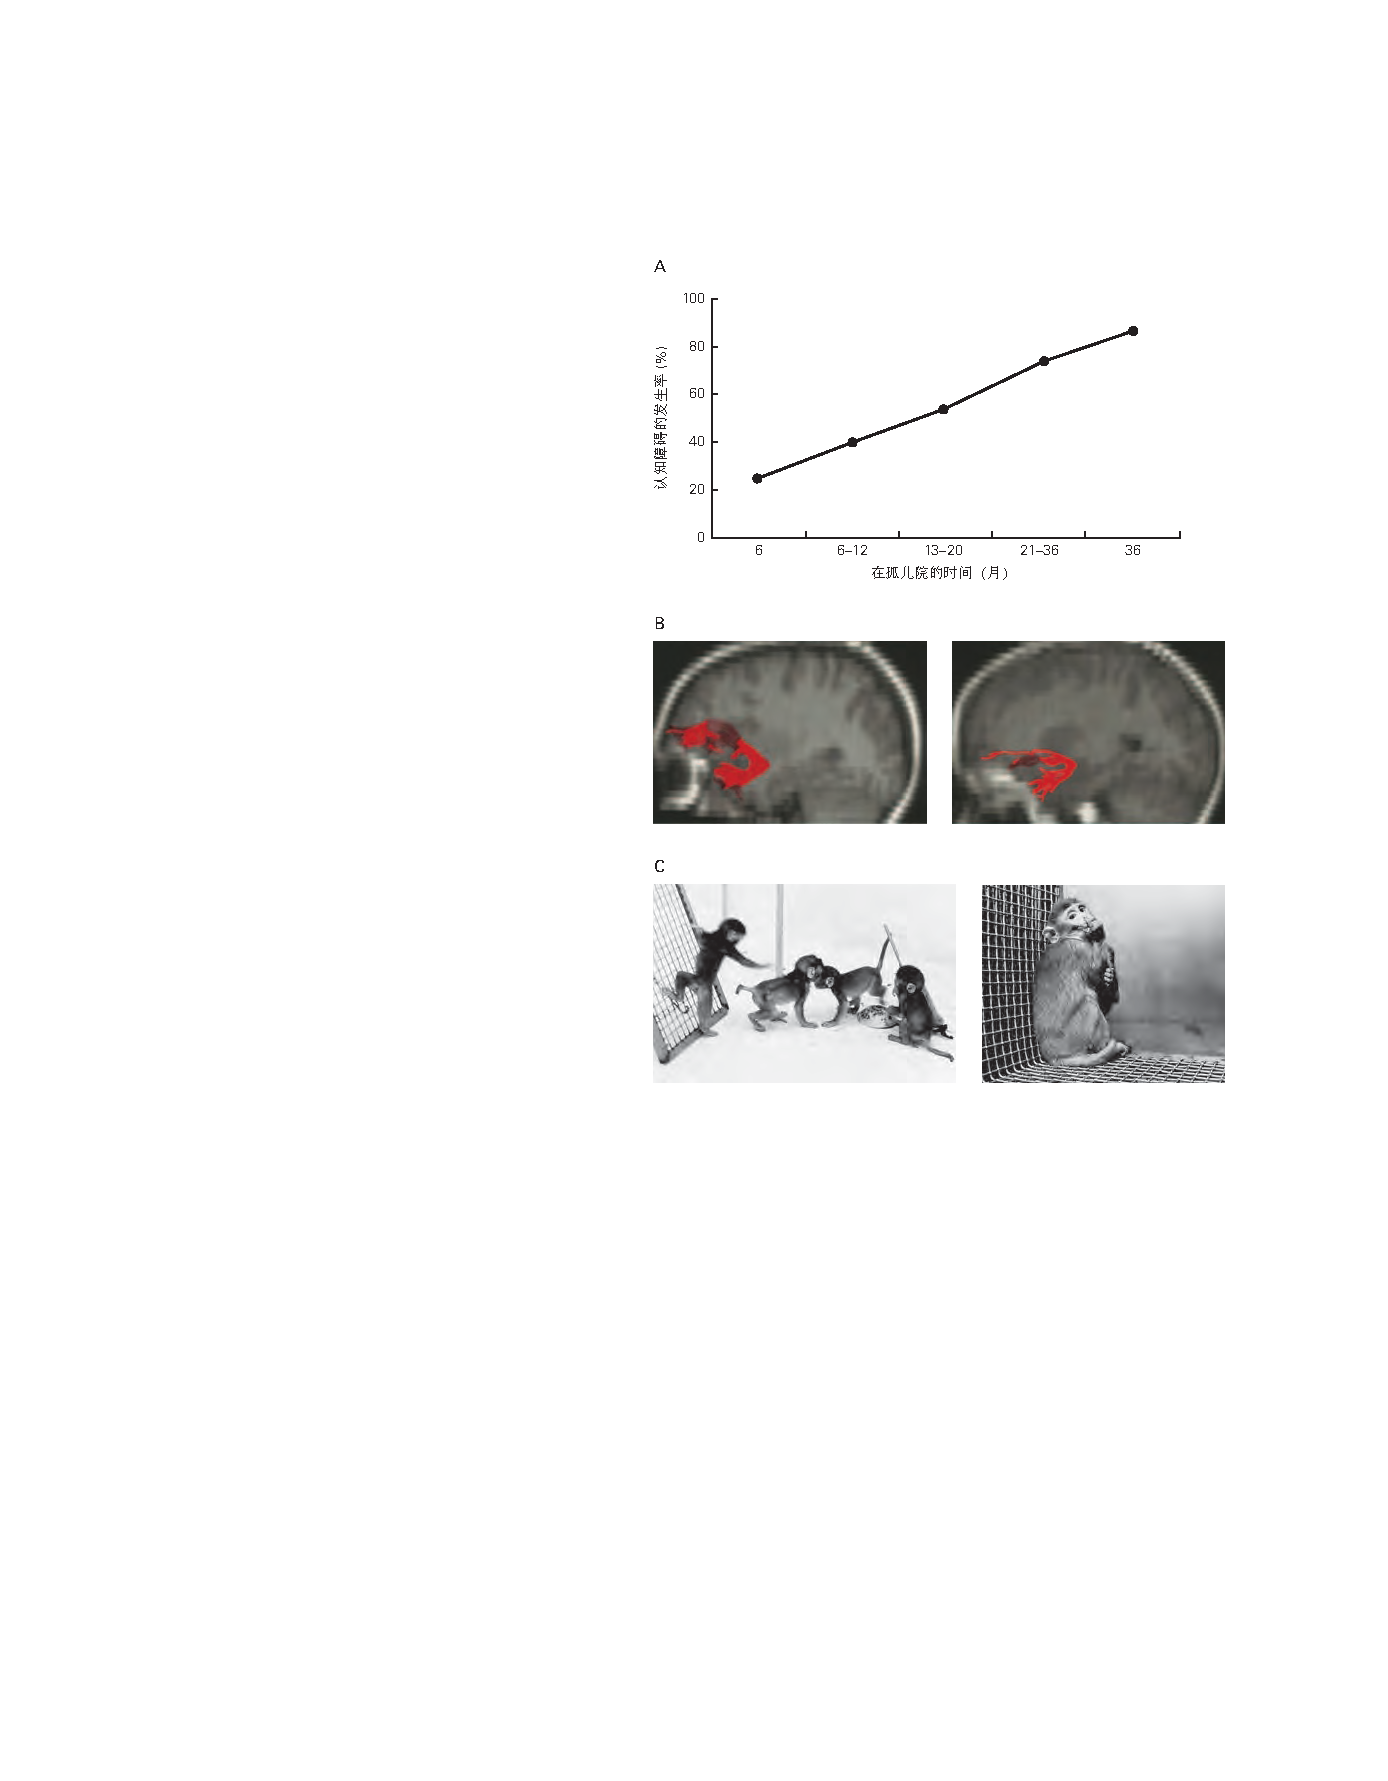
\includegraphics[width=0.89\linewidth]{chap49/fig_49_1}
	\caption{早期的社会剥夺对后来的大脑结构和行为有深远的影响。
		\textbf{A.} 在孤儿院社会剥夺条件下长大的儿童明显存在神经认知功能障碍。
		认知障碍的发生率随着在孤儿院逗留时间的延长而增加\cite{behen2008incidence}。
		\textbf{B.} 弥散张量\textit{核磁共振成像}扫描显示正常儿童(左)发育良好且强壮的钩束(红色区域),而社会剥夺儿童(右) ), 它很薄而且组织不善\cite{eluvathingal2006abnormal}。
		\textbf{C.} 早期社会互动影响后期社会行为模式。
		在兄弟姐妹在场的情况下饲养的猴子获得了社交技能,可以在以后的生活中进行有效的互动(左)。
		孤立地饲养的猴子永远无法获得与他人互动的能力,并且在以后的生活中仍然与世隔绝(右)。}
	\label{fig:49_1}
\end{figure}


尽管这些观察结果令人信服,但很难从中得出明确的结论。
1960 年代,两位心理学家\textit{哈里}和\textit{玛格丽特$\cdot$哈洛}进行了一组有影响力的研究,将社会行为分析扩展到猴子。
\textit{哈洛斯}将新生的猴子隔离饲养了 6 到 12 个月,剥夺了它们与母亲、其他猴子或人的接触。
在此期间结束时,猴子身体健康但行为受到破坏。 他们蹲在笼子的一角,像孤独症儿童一样来回摇晃(图~\ref{fig:49_1}C)。
它们不与其他猴子互动,也不打架、玩耍或表现出任何性兴趣。
因此,在出生后的前 18 个月里,为期 6 个月的社会隔离期会导致持续和严重的行为障碍。
相比之下,发现在可比较的时期内隔离年长的动物并没有造成如此严重的后果。
这些结果证实,在受控条件下,早期经验对后来行为的关键影响。
出于伦理原因,这些研究在今天是不可能的。



\subsection{视觉感知的发展需要视觉体验}

大脑对经验的极大依赖以及经验塑造感知的能力在先天性白内障患者中很明显。
白内障是晶状体混浊,会干扰眼睛的光学系统,但不会直接影响神经系统;
它们很容易通过手术切除。
在 1930 年代,很明显,患有先天性双眼白内障的患者在 10 岁后会出现永久性视力缺陷,并且难以感知形状和形态。
相比之下,当成人白内障在形成数十年后被移除时,正常视觉会立即恢复。


同样,患有斜视(斜视)的儿童没有正常的深度知觉(立体视觉),这种能力需要两只眼睛同时聚焦在同一位置。
如果他们的眼睛在生命的头几年通过手术矫正,他们就能获得这种能力,但如果在青春期后期进行手术,则不会。
由于这些观察结果,现在通常会在儿童早期切除先天性白内障,并通过手术矫正斜视。
在过去的五年中,研究人员阐明了这些关键时期的结构和生理基础。



\section{视觉皮层双眼回路的发育取决于产后活动}

由于对世界的感官体验会转化为大脑中的电活动模式,因此可以想象神经回路中的电信号会影响大脑的回路。
但这是真的吗?
如果这是真的,会发生什么变化,活动如何触发它们?


我们对这些联系的最详细理解来自对调节双眼视觉的神经回路的研究。
这项工作早期阶段的关键人物是\textit{大卫$\cdot$休伯尔}和\textit{托斯坦$\cdot$威泽尔}。
在对猫和猴子视觉皮层的结构和功能组织进行开创性研究后(第~\ref{chap:chap23}~章),他们又进行了另一组研究,研究经验如何影响他们所描述的回路。



\subsection{视觉体验影响视觉皮层的结构和功能}

在一项有影响力的研究中,\textit{休伯尔}和\textit{威泽尔}将一只猴子从出生养到 6 个月大,一只眼睑被缝合,从而剥夺了动物那只眼睛的视力。
当缝合线被拆除时,很明显这只动物被剥夺的眼睛是盲的,这种情况称为弱视。
然后,他们对视觉通路沿线的细胞进行电生理记录,以确定缺陷出现的位置(图~\ref{fig:49_2})。
他们发现被剥夺的眼睛中的视网膜神经节细胞,以及从被剥夺的眼睛接收输入的外侧膝状体核中的神经元,对视觉刺激反应良好,并且具有基本正常的感受野。


\begin{figure}[htbp]
	\centering
	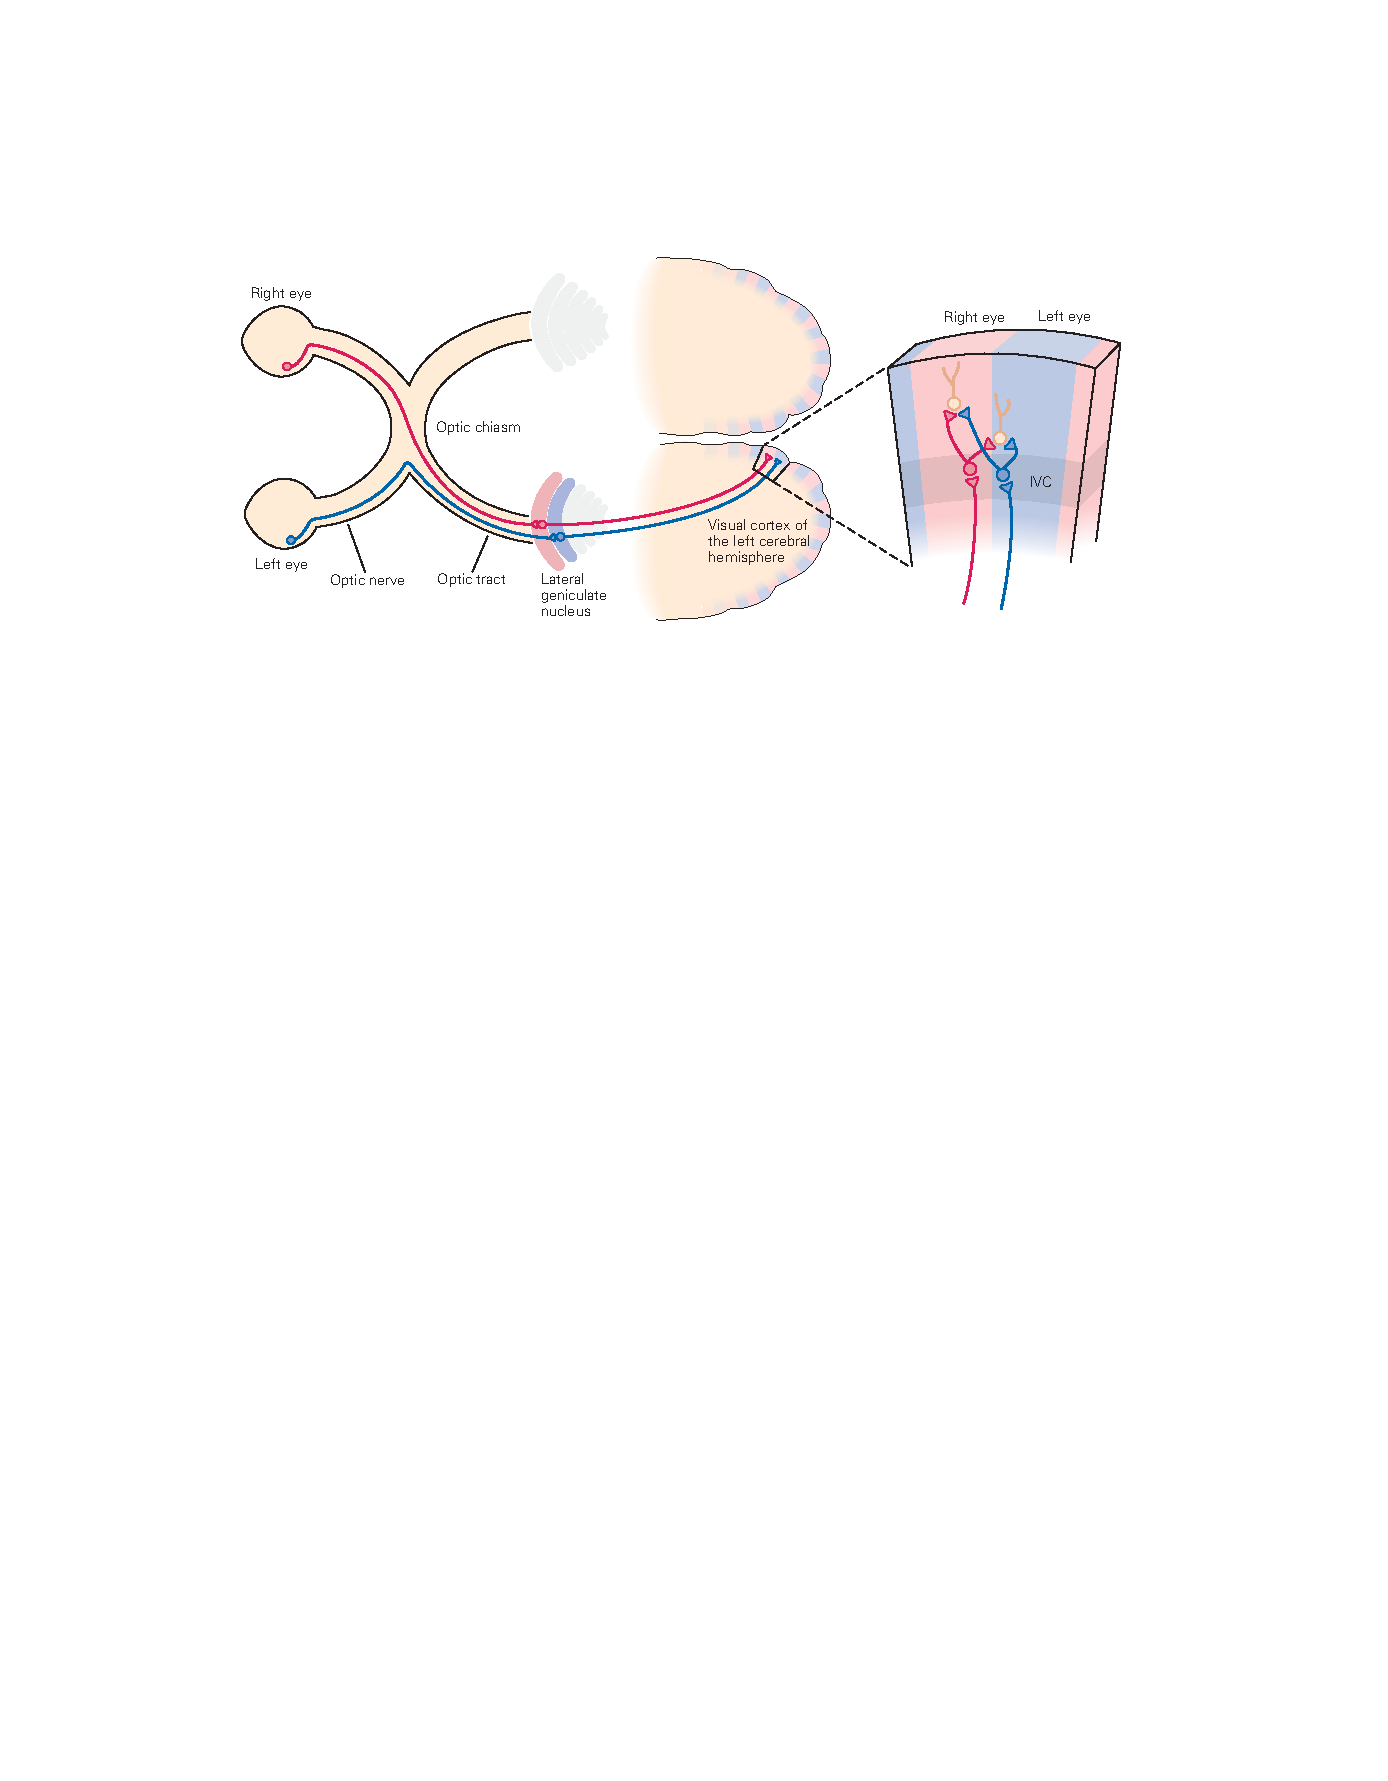
\includegraphics[width=1.0\linewidth]{chap49/fig_49_2}
	\caption{来自两只眼睛的传入通路投射到视觉皮层中离散的神经元柱。
		来自每只眼睛的视网膜神经节神经元将轴突发送到外侧膝状体的不同层。
		该核中神经元的轴突投射到初级视觉皮层\textit{岛前庭皮层}层中的神经元,该层组织成交替的眼优势柱组;
		每列仅接收来自一只眼睛的输入。
		\textit{岛前庭皮层}层神经元的轴突投射到相邻列的神经元以及同一列上下层的神经元。
		结果,皮层上层和下层的大多数神经元都从双眼接收信息。}
	\label{fig:49_2}
\end{figure}


相反,视觉皮层中的细胞发生了根本性的改变。
在正常动物的皮层中,大多数神经元对双眼输入有反应。
在前 6 个月被单眼剥夺的动物中,大多数皮层神经元对来自被剥夺眼睛的信号没有反应(图~\ref{fig:49_3})。
少数有反应的皮层细胞不足以进行视觉感知。
被剥夺的眼睛不仅失去了驱动大多数皮层神经元的能力,而且几乎没有恢复:
这种损失是永久性的,不可逆转的。


\begin{figure}[htbp]
	\centering
	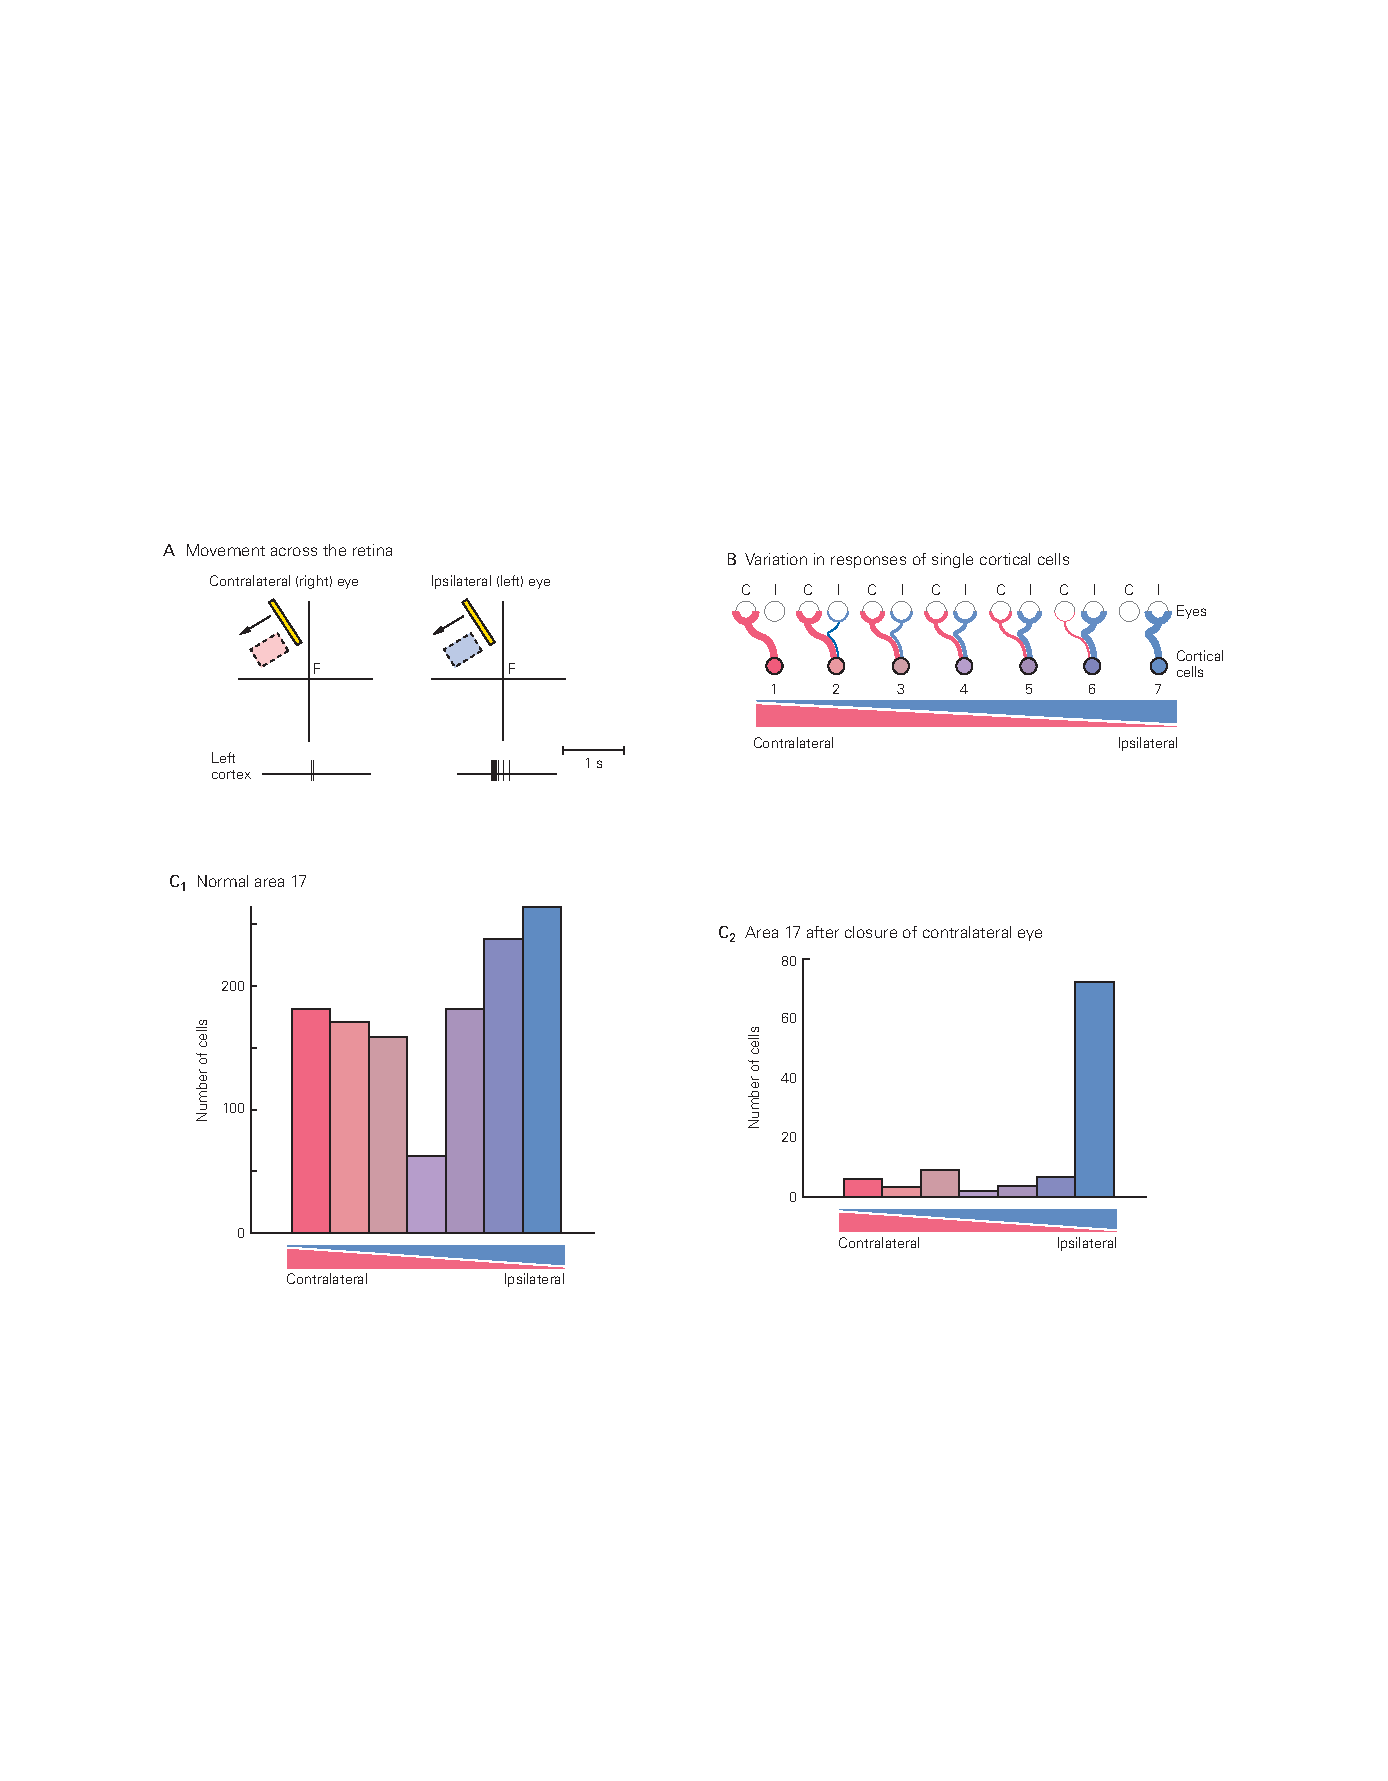
\includegraphics[width=1.0\linewidth]{chap49/fig_49_3}
	\caption{猴子初级视觉皮层神经元对视觉刺激的反应\cite{hubel1977ferrier}。
		\textbf{A.} 一条对角线光条向左移动穿过视野,穿过视觉皮层区域 17 中双眼反应细胞的感受野。
		分别绘制通过右眼和左眼测量的感受野。
		两个细胞的感受野在方向、位置、形状和大小上都相似,并对相同形式的刺激做出反应。
		记录(下图)显示皮层神经元对来自同侧眼睛的输入反应更有效。
		\textbf{B.} 区域 17 中单个皮层神经元的反应可分为七组。
		仅从对侧眼(C)接收输入的神经元属于第 1 组,而仅从同侧眼(I)接收输入的神经元属于第 7 组。
		其他神经元从双眼接收输入,但来自一只眼睛的输入可能会比另一个神经元(第 2 组和第 6 组)影响多得多,或者差异可能很小(第 3 组和第 5 组)。
		一些神经元对双眼的输入反应相同(第 4 组)。
		根据这些标准,A 部分所示的皮层神经元属于第 6 组。
		\textbf{C.} 区域 17 中的神经元对一只或另一只眼睛的刺激的相应。
		1.正常成年和幼猴左半球 17 区 1 千多个神经元的反应。
		通常仅接收单眼输入的第 IV 层神经元已被排除在外。
		2. 猴子左半球神经元的相应,其中对侧(右)眼从 2 周龄到 18 个月大时闭上,然后再睁开。
		大多数神经元仅对同侧眼的刺激有反应。}
	\label{fig:49_3}
\end{figure}


\textit{休伯尔}和\textit{威泽尔}继续测试了不同年龄段的较短时间视觉剥夺的影响。
根据剥夺的时间和持续时间,他们获得了三种类型的结果。
首先,出生后不久的几周单眼剥夺导致被剥夺的眼睛失去皮层反应,这在眼睛打开后是可逆的,特别是如果另一只眼睛随后关闭以鼓励使用最初被剥夺的眼睛。
其次,在接下来的几周内持续几周的单眼剥夺也导致皮层对来自被剥夺的眼睛的信号的反应性显著丧失,但在这种情况下,影响是不可逆转的。
最后,成人的剥夺,即使是数月的时间,也不会影响皮层细胞对来自被剥夺眼睛的信号或视觉感知的反应。
这些结果表明,控制视觉感知的皮层连接是在早期发育的关键时期建立的。


这些功能缺陷是否存在解剖学相关性?
为了解决这个问题,我们需要回顾关于视觉皮层解剖结构的三个基本事实(图~\ref{fig:49_2})。
首先,来自两只眼睛的输入在外侧膝状体核中保持分离。
其次,将信息从两只眼睛传送到皮层的膝状体输入终止于交替的列,称为眼优势列。
第三,外侧膝状体轴突终止于初级视觉皮层\textit{岛前庭皮层}层的神经元;
两只眼睛在共同目标细胞上的输入会聚发生在通路的下一阶段,在\textit{岛前庭皮层}层上方和下方的细胞中。


为了检查眼优势柱的结构是否依赖于出生后早期的视觉体验,\textit{休伯尔}和\textit{威泽尔}剥夺了新生动物一只眼睛的视力,然后将一种标记的氨基酸注射到正常的眼睛中。
注入的标记被整合到视网膜神经节细胞体中的蛋白质中,沿着视网膜轴突输送到外侧膝状体核,转移到膝状体神经元,然后输送到初级视觉皮层中这些轴突的突触末端。
闭上一只眼睛后,从被剥夺的眼睛传递输入的突触末端柱状阵列减少,而从正常眼睛传递输入的柱状末端阵列扩大(图~\ref{fig:49_4})。
因此,生命早期的感觉剥夺会改变大脑皮层的结构。


\begin{figure}[htbp]
	\centering
	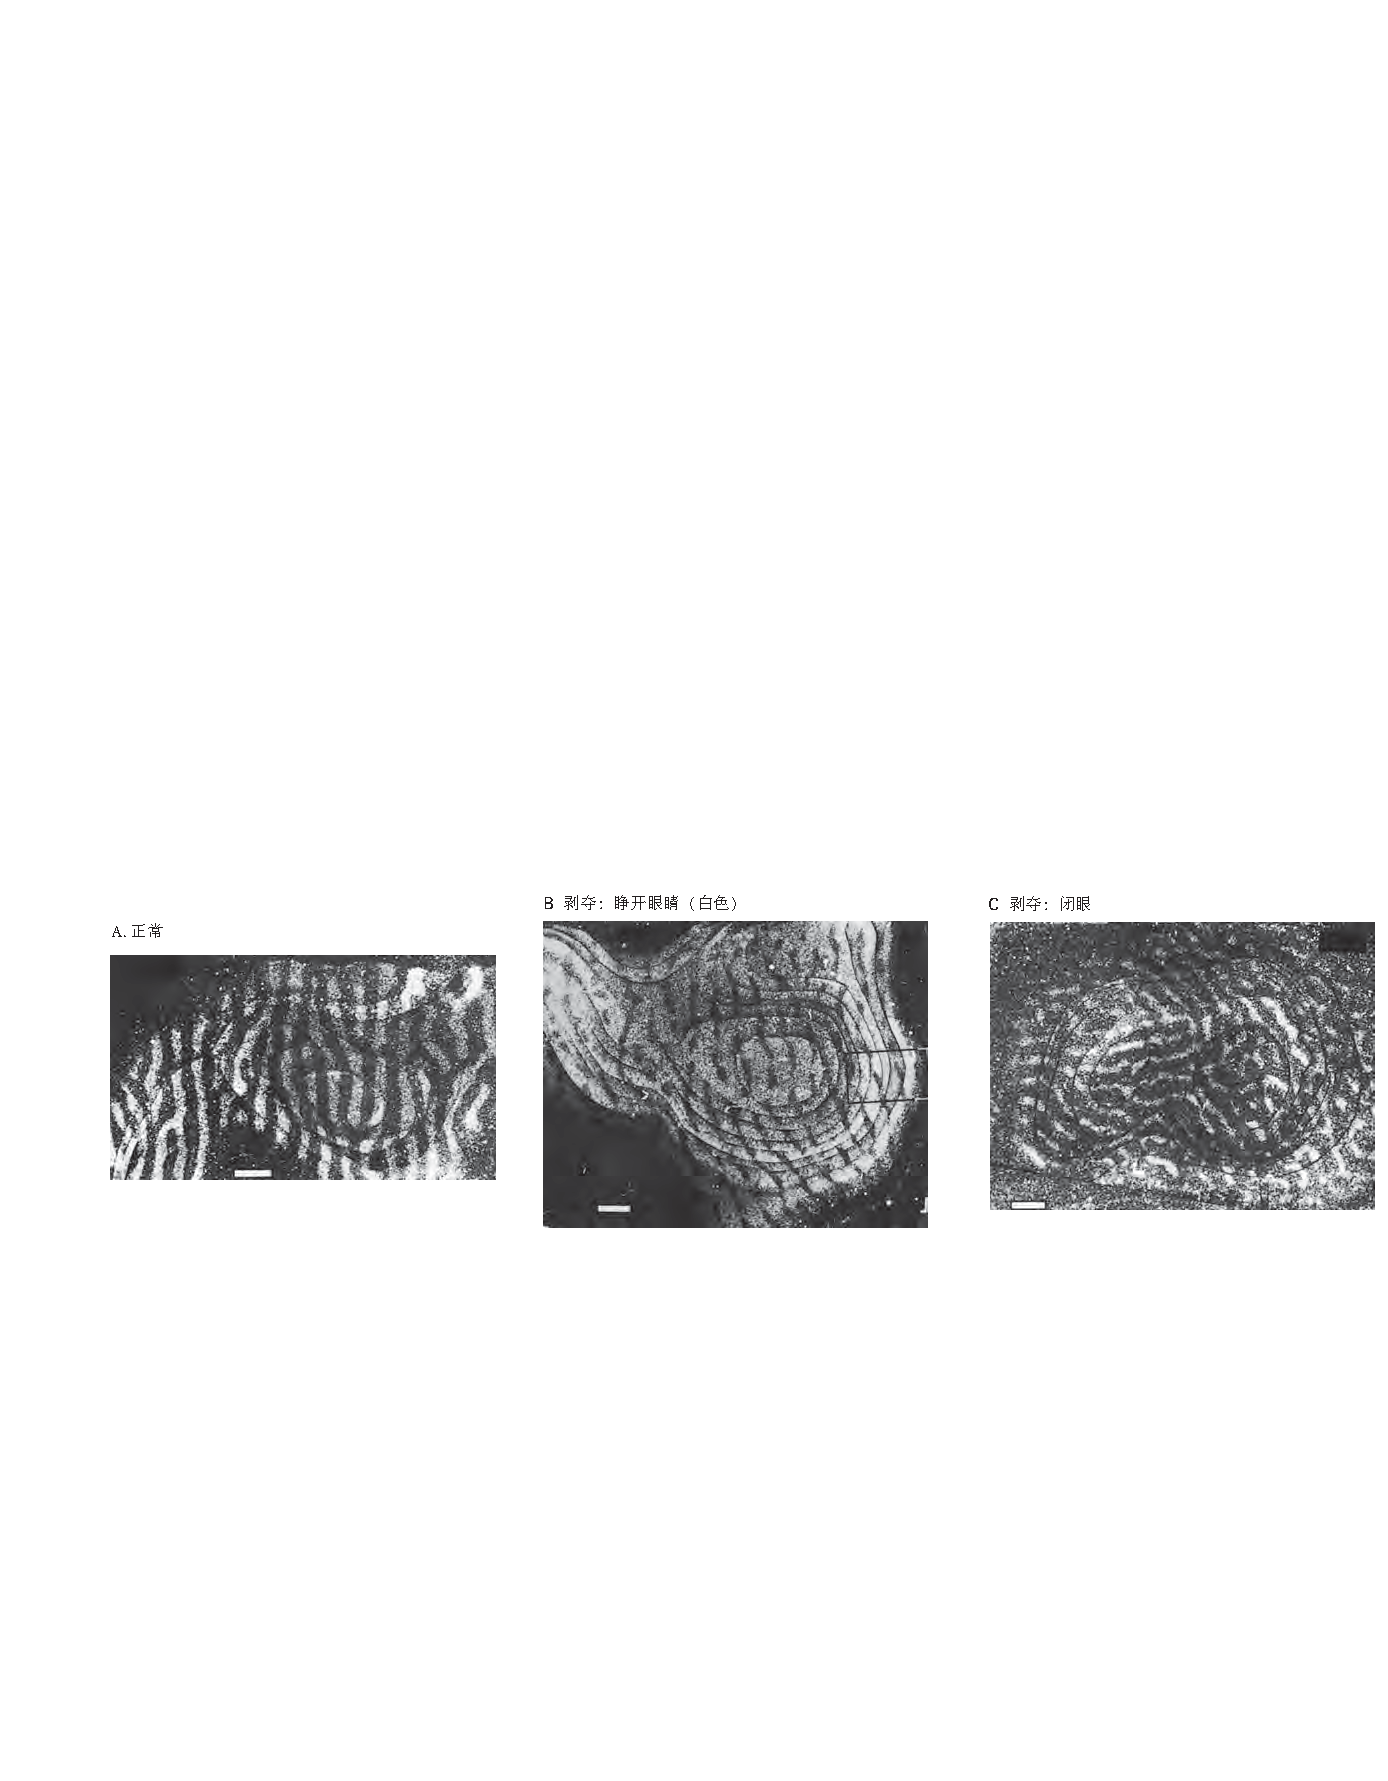
\includegraphics[width=1.0\linewidth]{chap49/fig_49_4}
	\caption{在发育的关键时期,一只眼睛的视觉剥夺会减少那只眼睛的眼优势列的宽度。
		(比例尺 = 1 毫米)\cite{hubel1977ferrier}
		\textbf{A.} 正常成年猴子右半球 17 区的切向切面,在一只眼睛注射放射性标记的氨基酸药物 10 天后。
		放射性位于视觉皮层\textit{岛前庭皮层}层的条纹(白色)中,表明来自外侧膝状体的轴突终止部位,该核携带来自注射眼的输入。
		交替的未标记(深色)条纹表示携带来自未注射眼睛的信号的轴突的终止部位。
		标记和未标记的条纹宽度相等。
		\textbf{B.} 一只 18 个月大的猴子的视觉皮层的类似切片,该猴子的右眼在 2 周大时通过手术闭合。
		将标签注射到左(睁)眼中。
		较宽的(白色)条纹是带有来自睁眼信号的传入轴突的标记末端; 窄(暗)条纹是轴突的末端,输入来自闭眼。
		\textbf{C.} 与 B 部分相当的部分来自一只 18 个月大的动物,其右眼在 2 周时被关闭。
		标签被注射到闭合的眼睛中,导致标记轴突末端的窄(白色)条纹和未标记末端的宽(暗)条纹。}
	\label{fig:49_4}
\end{figure}


这些惊人的解剖学变化是如何产生的?
感觉剥夺是否会在眼优势柱建立后改变它们,还是会干扰它们的形成?
视觉皮层的柱状组织在猴子出生时就已经很明显了,尽管成熟的模式要到出生后几周才能实现(图~\ref{fig:49_5})。
只有在这个时候,来自外侧膝状体核的纤维末端才会在皮层中完全分离。
由于在视觉剥夺发挥作用时输入部分但未完全隔离,我们可以得出结论,剥夺扰乱了输入获得其成熟模式的能力。
在本章的后面部分,我们将回到什么导致最初的、与经验无关的隔离阶段的问题。


\begin{figure}[htbp]
	\centering
	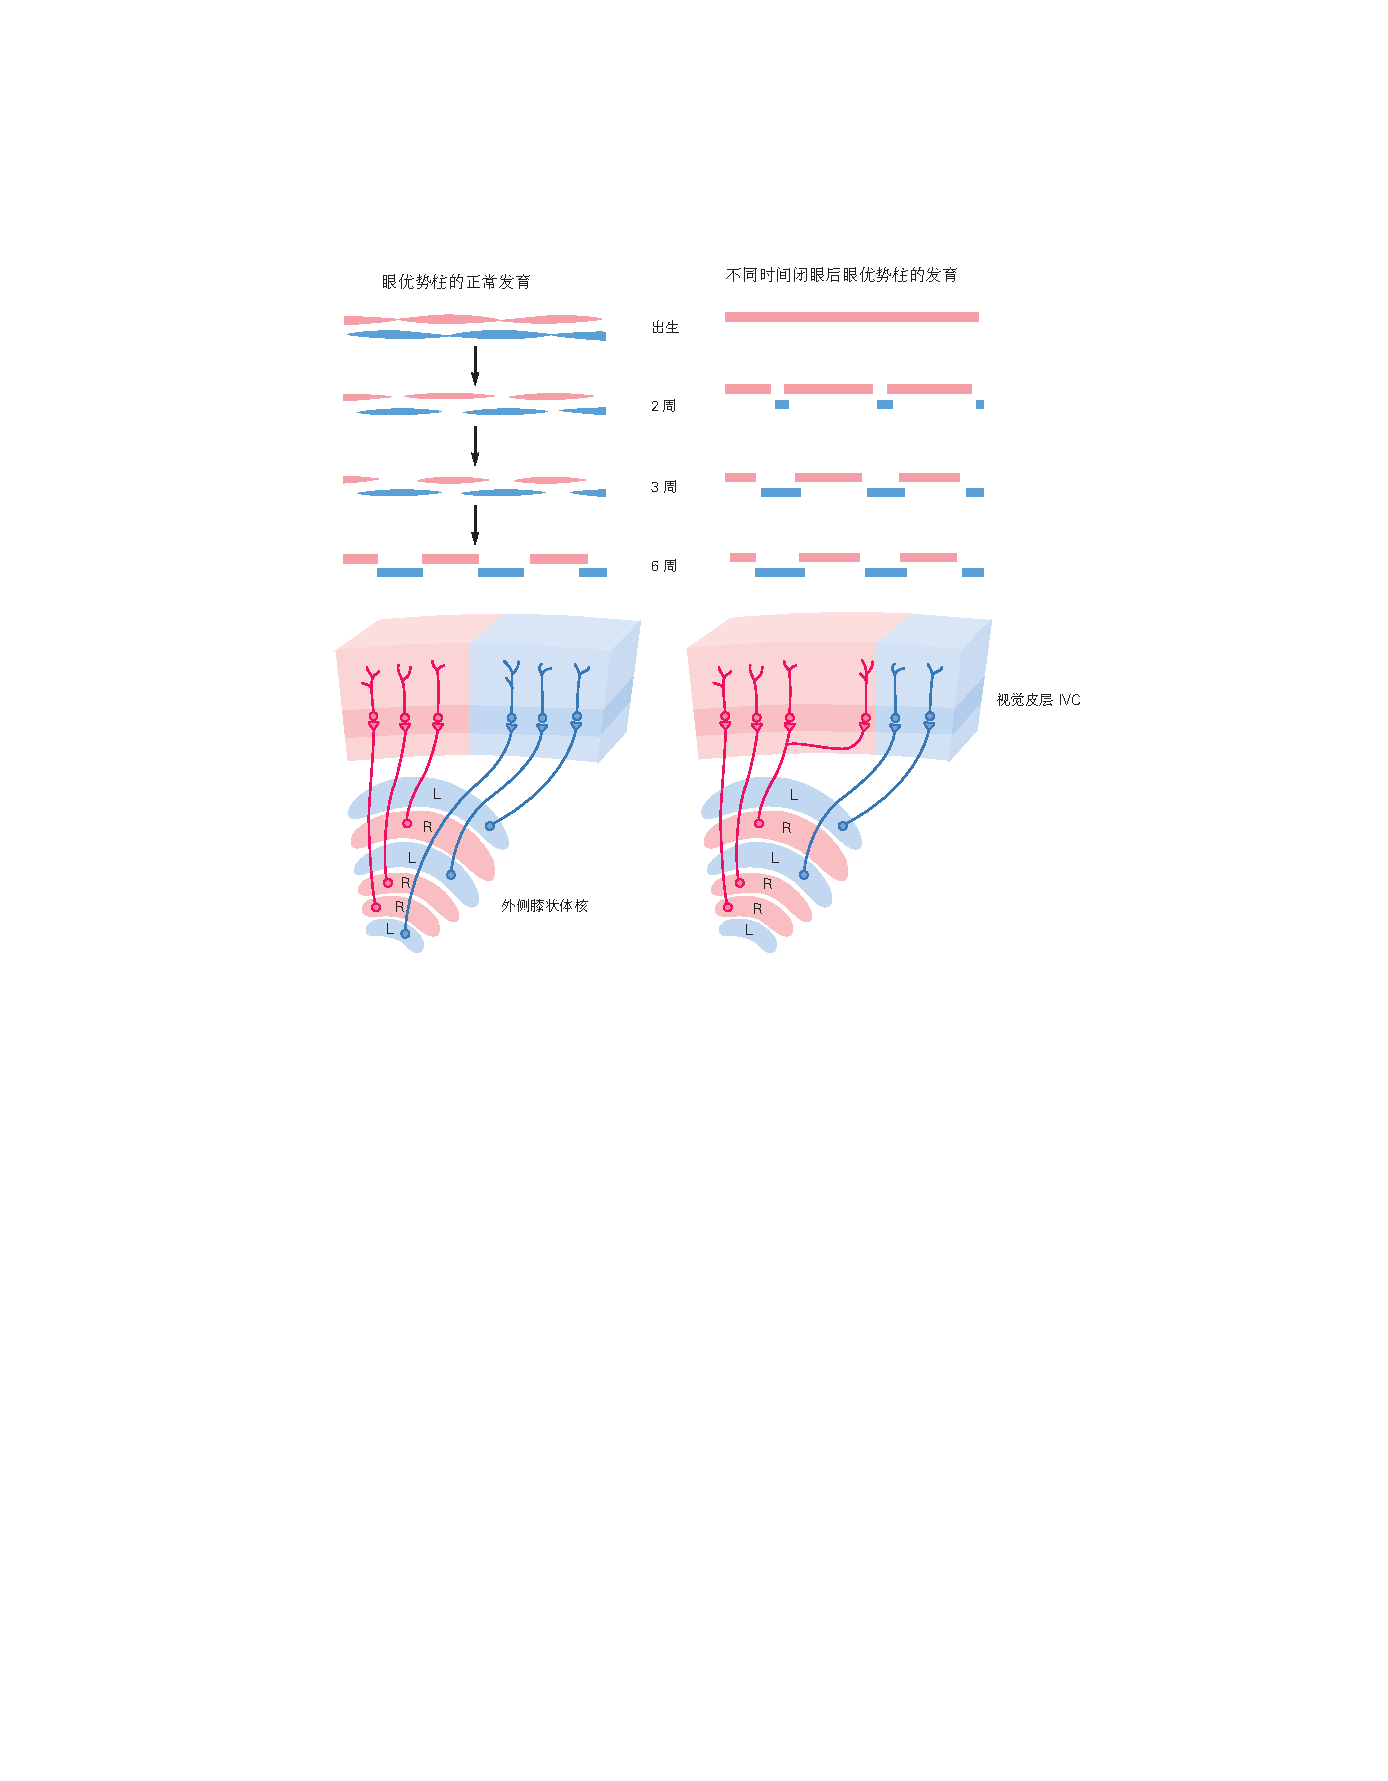
\includegraphics[width=0.98\linewidth]{chap49/fig_49_5}
	\caption{闭眼对眼优势柱形成的影响。
		上图显示在正常条件下(左)和一只眼睛被剥夺刺激(右)时,视觉皮层\textit{岛前庭皮层}层外侧膝状体传入神经末梢逐渐分离。
		蓝色区域代表一只眼睛的输入终止区域,红色区域代表另一只眼睛的输入区域。
		域的长度表示沿\textit{岛前庭皮层}层每个点的终端密度。
		为清楚起见,这些列在这里显示为一个在另一个之上,而实际上,它们在皮层中是并排的。
		在正常发育过程中,下腔静脉层逐渐分为每只眼睛的交替输入部位。
		一只眼睛失明的后果取决于闭眼的时间。
		出生时闭合导致睁眼(红色)占主导地位,因为此时几乎没有发生隔离。
		在第 2、3 和 6 周关闭对眼优势柱的形成的影响逐渐减弱,因为这些柱随着时间变得更加分离\cite{hubel1977ferrier}。 }
	\label{fig:49_5}
\end{figure}


\subsection{电活动的模式组织双眼回路}

活动如何导致眼优势柱的成熟?
关键因素可能是出生时每只眼睛汇聚在共同目标细胞上的输入比例的差异。
如果碰巧从一只眼睛传送输入的纤维最初在皮层的一个局部区域更多,那么这些轴突可能具有优势,导致进一步分离。


这怎么可能发生?
基于\textit{唐纳德$\cdot$赫布}在 1940 年代首次提出的理论,一个有吸引力的想法是,当突触前和突触后元素一起活跃时,突触连接会得到加强。
在双眼相互作用的情况下,来自同一只眼睛的相邻轴突往往会同步发射,因为它们在任何瞬间都被相同的视觉刺激激活。
它们发射的同步意味着它们在靶细胞的去极化和激发中协同作用。
这种合作行为以非合作突触为代价维持了这些突触联系的可行性。


合作活动还可以促进轴突的分支,从而为与目标区域中的细胞形成额外的突触连接创造机会。
同时,一只眼睛的轴突加强突触接触会阻碍另一只眼睛的突触输入的增长。
从这个意义上讲,可以说来自两只眼睛的纤维在争夺目标细胞。
轴突之间的合作和竞争共同确保两个传入纤维群最终将支配初级视觉皮层的不同区域,几乎没有局部重叠。


竞争与合作不仅仅是神经活动本身或轴突之间绝对活动水平差异的结果。
相反,它们似乎依赖于竞争(或合作)轴突中精确的时间活动模式。
\textit{休伯尔}和\textit{威泽尔}在一组检查立体视觉(深度感知)的研究中生动地说明了这一原理。
大脑通常通过比较两只眼睛之间视网膜图像的差异来计算深度感知。
当眼睛没有正确对准时,就无法进行这种比较,也就不可能进行立体观察。
这种错位发生在“斗鸡眼”或斜视的儿童身上。
如上所述,这种情况可以通过手术修复,但除非手术发生在生命的最初几年,否则孩子们将永远无法进行立体观察


\textit{休伯尔}和\textit{威泽尔}研究了斜视对猫视觉系统组织的影响。
为了使猫斜视,小猫的眼外肌肌腱被切断。 两只眼睛都保持完好功能,但没有对齐。
来自两只眼睛的输入会聚在视觉皮层的双眼细胞上,现在携带了关于视野略有不同部分的不同刺激的信息。
结果,皮层细胞变成了单眼细胞,由一只眼睛或另一只眼睛而非两只眼睛的输入驱动(图~\ref{fig:49_6})。 
相反,皮层神经元在双眼视觉剥夺后仍保持双眼反应,导致双眼活动减少但不会失衡。
这些发现向\textit{休伯尔}和\textit{威泽尔}表明,输入同步性的中断会导致竞争而不是合作,因此皮层细胞开始由一只眼睛支配,大概是一开始支配的那只眼睛。


\begin{figure}[htbp]
	\centering
	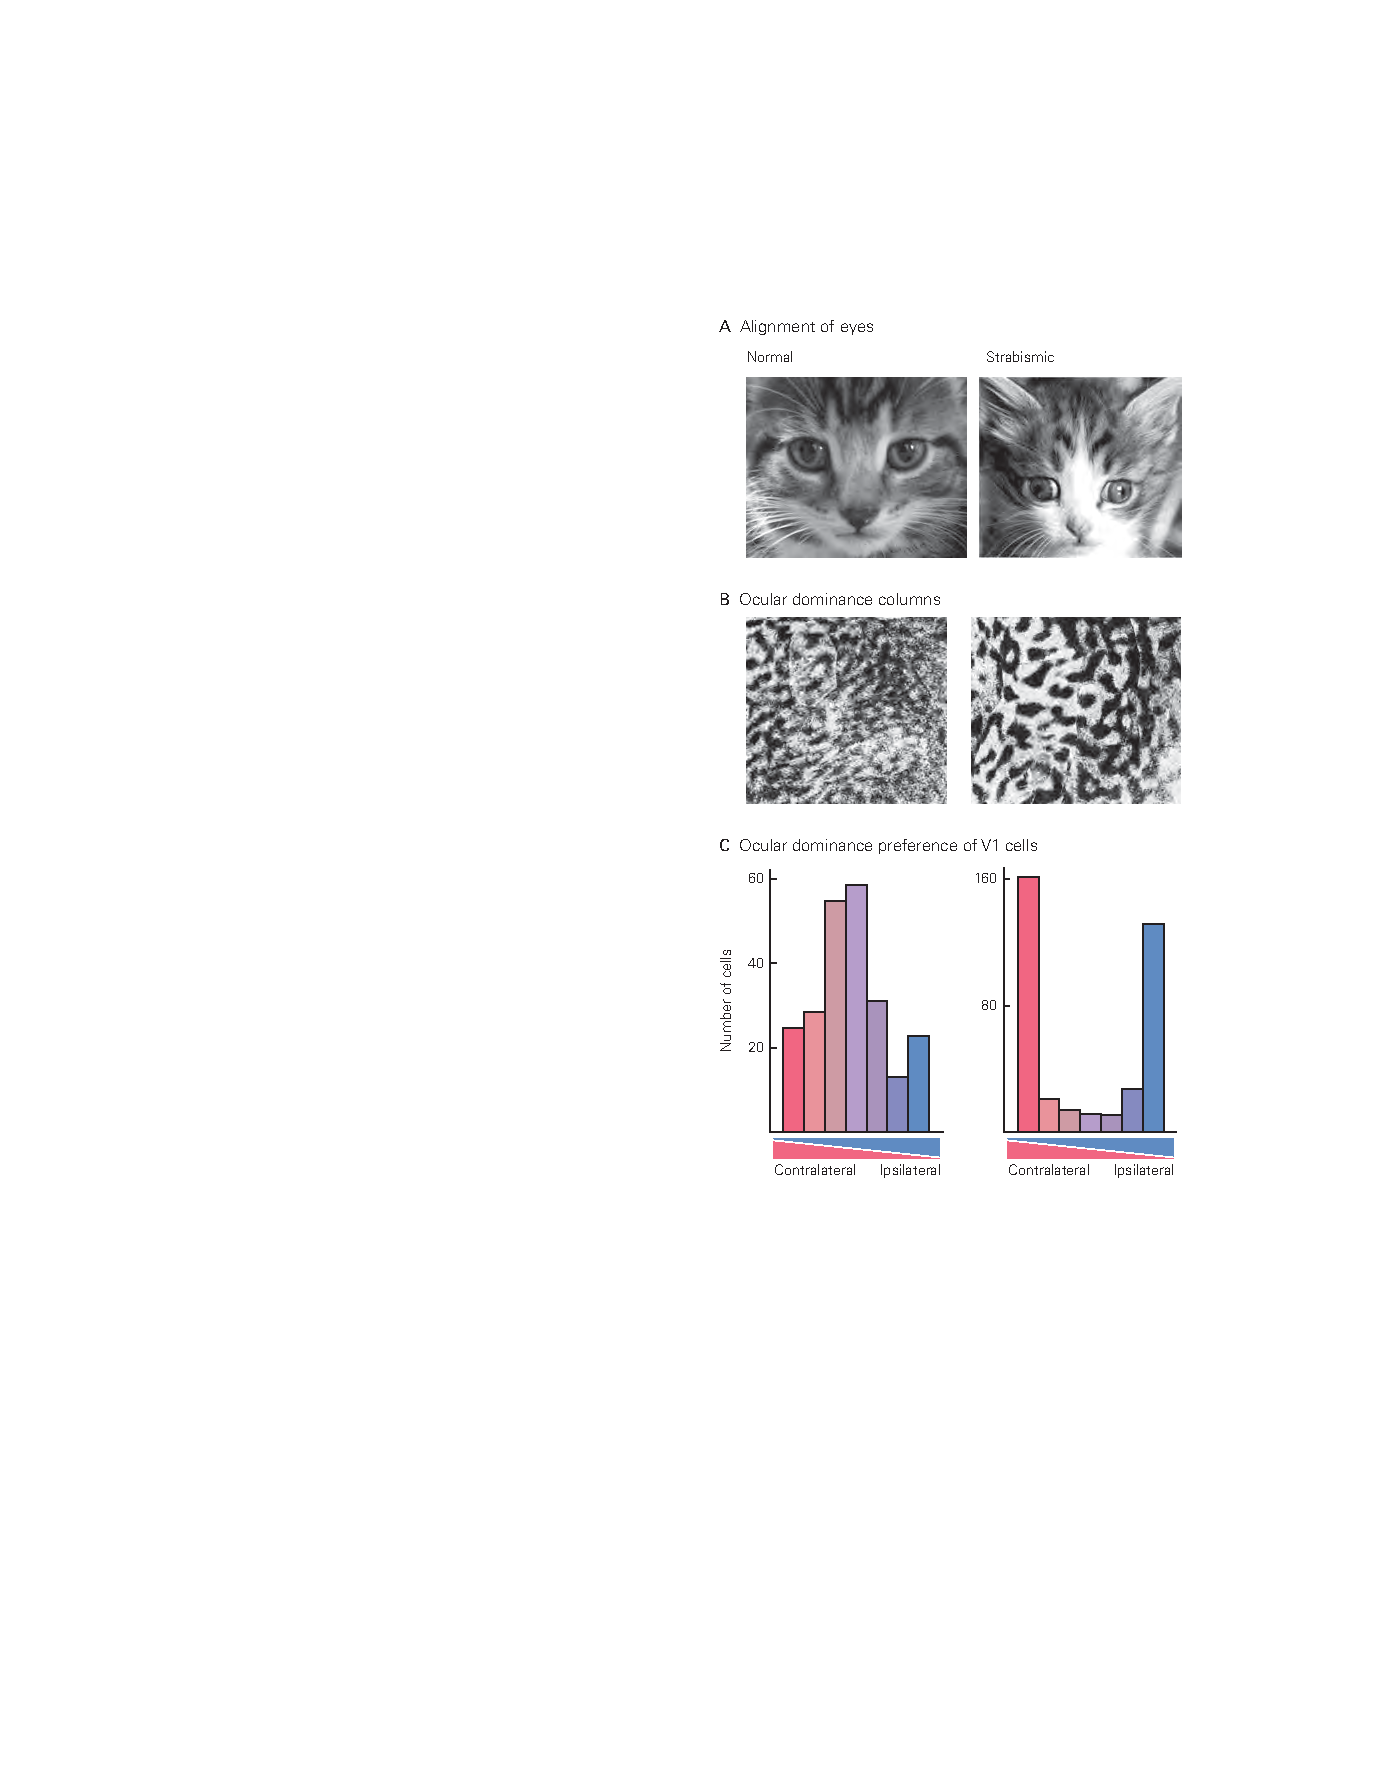
\includegraphics[width=0.8\linewidth]{chap49/fig_49_6}
	\caption{在小猫中诱发斜视会损害初级视觉皮层中双眼反应区域的形成。
		\textbf{A.} 斜视猫的眼睛是错位的。
		\textbf{B.} 在斜视动物中,左眼和右眼区域更清晰,表明双眼区域缺乏。
		\textbf{C.} 斜视动物在视觉皮层中的双眼调谐神经元较少。}
	\label{fig:49_6}
\end{figure}


这些生理学研究促使研究人员测试视网膜神经节细胞电活动的药理学阻断是否会影响视觉系统中的神经连接。
通过向双眼注射河豚毒素来阻断活性,河豚毒素是一种选择性阻断电压敏感 \ce{Na+} 通道的毒素。
来自两只眼睛的信号是通过对双侧视神经的直接电刺激分别产生的。
在小猫中,如果视网膜神经节神经元的活动在发育的关键时期之前被阻断,则不会建立眼优势柱。
当两条视神经同时受到刺激时,眼优势柱仍未能形成。
只有当视神经被异步刺激时,才会建立眼优势列。


如果眼优势柱的发展确实依赖于两只眼睛纤维之间的竞争,是否有可能通过在两组轴突之间建立竞争来诱导通常不存在的柱的形成?
这种激进的可能性在青蛙身上进行了测试,青蛙每只眼睛的视网膜神经节神经元仅投射到大脑的对侧。
在正常的青蛙中,来自两只眼睛的传入纤维不会竞争相同的细胞,因此传入输入不存在柱状分离。
为了产生竞争,第三只眼睛在幼虫发育的早期被移植到青蛙头部靠近一只正常眼睛的区域。
额外眼睛的视网膜神经节神经元将轴突延伸至对侧视顶盖。
值得注意的是,移植眼和正常眼的轴突末端分离,产生交替柱状图案(图~\ref{fig:49_7})。


\begin{figure}[htbp]
	\centering
	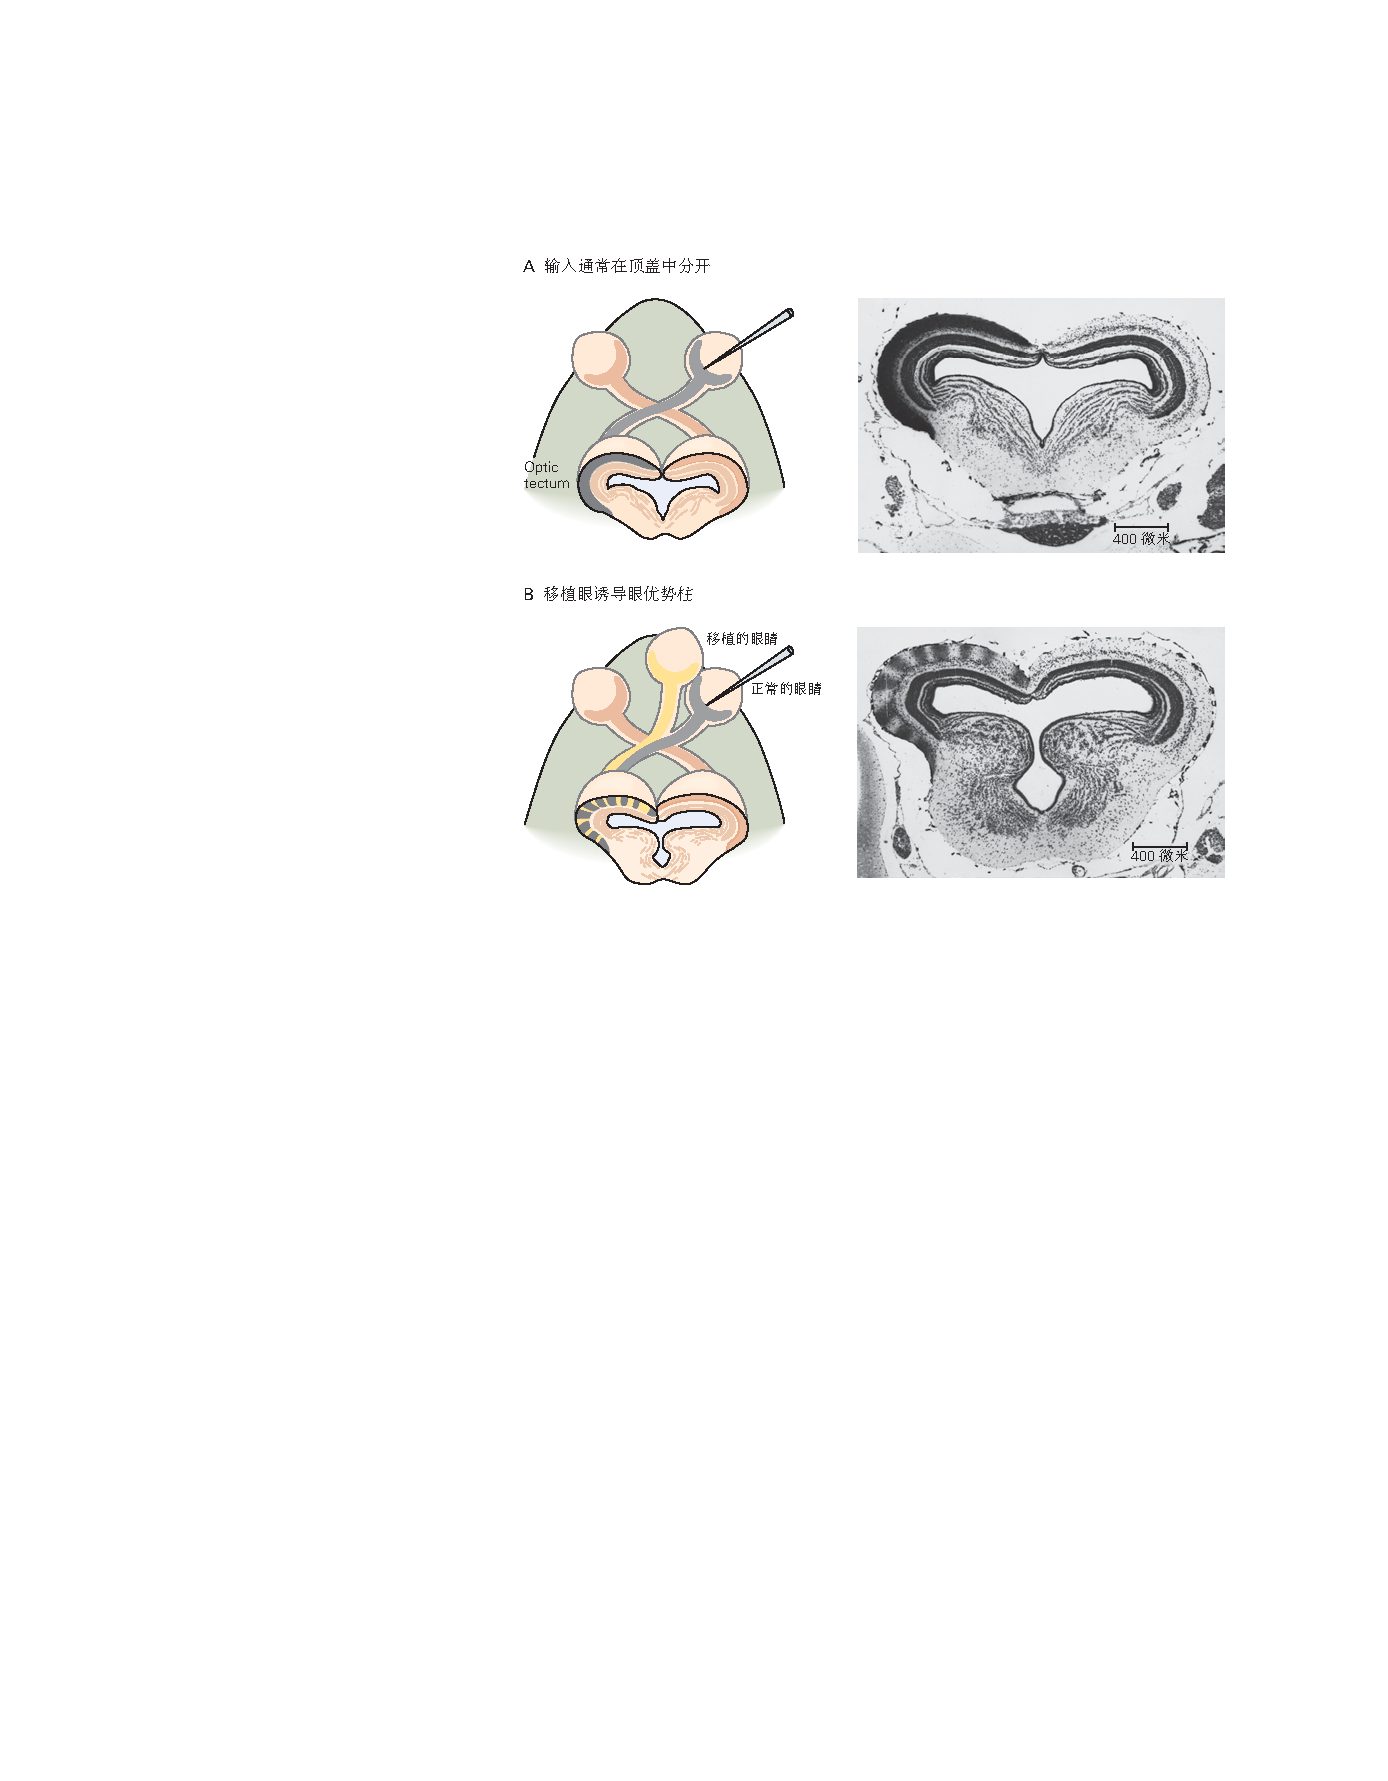
\includegraphics[width=0.79\linewidth]{chap49/fig_49_7}
	\caption{可以通过移植第三只眼在青蛙中实验性地诱导眼优势柱\cite{constantine1978eye}。
		\textbf{A.} 移植前三天,右眼注射了放射性标记的氨基酸。
		后脑冠状切面的放射自显影照片显示左侧视叶的整个浅表神经细胞都充满了银颗粒,表明标记(对侧)眼的突触末梢占据的区域。
		\textbf{B.} 在第三只眼被移植到正常右眼附近一段时间后,右眼被注射了放射性标记的氨基酸。
		放射自显影图显示左侧视叶接收来自标记眼和移植眼的输入。
		对侧眼通常连续的突触区已分为交替的暗区和亮区,指示每只眼睛的输入位置。}
	\label{fig:49_7}
\end{figure}


这一发现极大地支持了这样一种观点,即传入轴突之间对同一目标神经元群的竞争促使它们分离到不同的目标区域。
青蛙大脑中视网膜输入的柱状分离取决于突触活动,大概是在视网膜轴突和顶盖神经元之间的突触处。
因此,神经活动在微调视觉回路中具有强大的作用。



\section{关键时期视觉回路的重组涉及突触连接的改变}

\textit{休伯尔}、\textit{威泽尔}及其同事的开创性工作表明,视觉皮层正常结构和功能的出现需要早期经验。
然而,构成关键期的细胞和分子机制仍然是个谜。
近年来,许多调查人员开始着手解决这些问题。
他们的大部分工作都涉及到使用老鼠,因为老鼠比\textit{休伯尔}、\textit{威泽尔}和他们的弟子研究的猫和猴子更容易进行机械分析。


\subsection{皮层重组取决于兴奋和抑制的变化}

与猫和猴子不同,大多数小鼠视觉皮层仅接收对侧输入,其双眼区域不分为眼优势列。
尽管如此,小双眼区域包含单眼和双眼驱动神经元的混合物,并且在眼优势的关键时期关闭对侧眼显著地将双眼神经元的偏好转移到来自同侧眼的输入(图~\ref{fig:49_8})。


\begin{figure}[htbp]
	\centering
	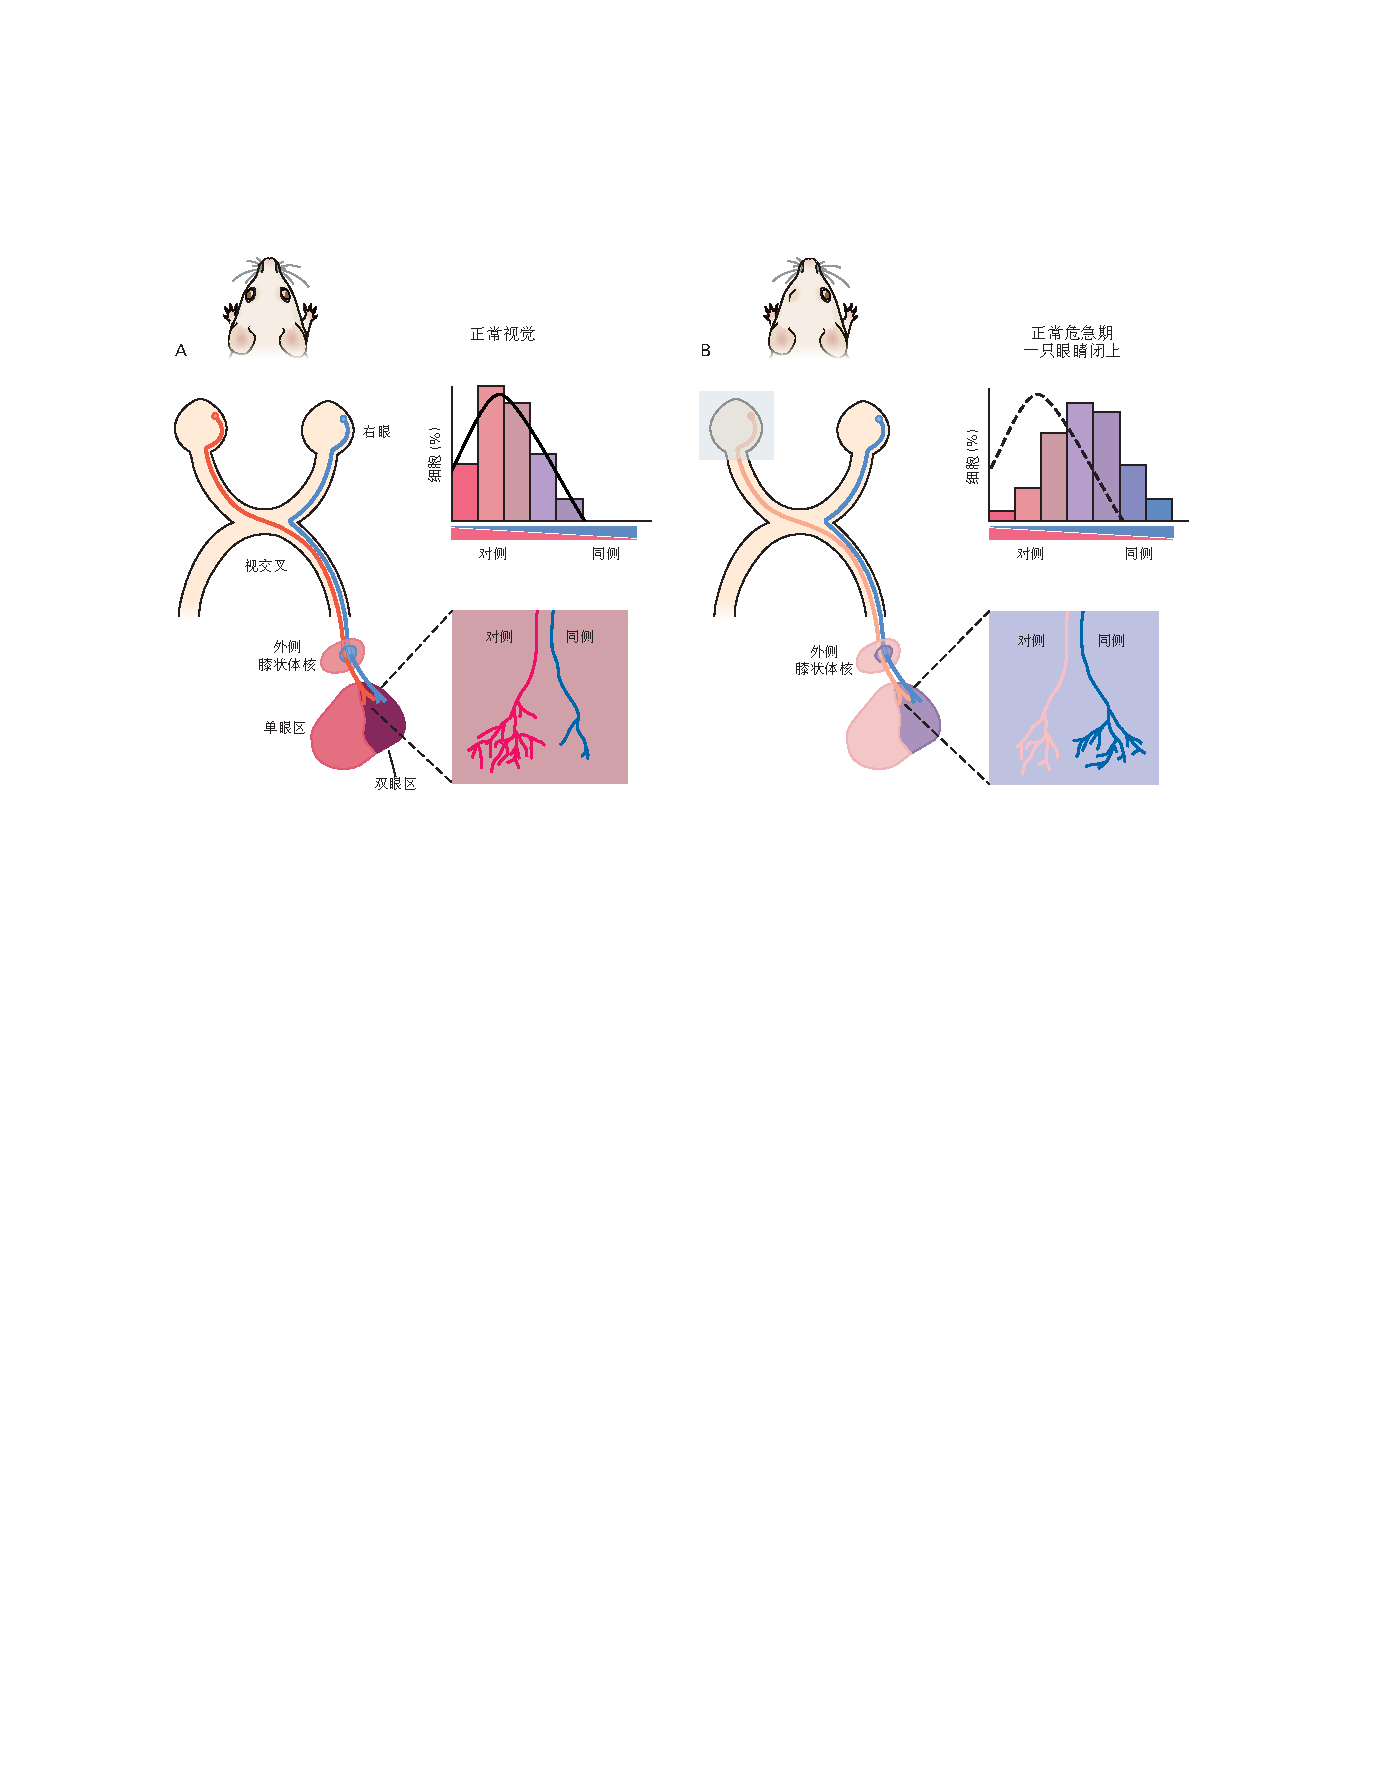
\includegraphics[width=1.0\linewidth]{chap49/fig_49_8}
	\caption{眼优势可塑性的关键时期在小鼠身上很明显\cite{hensch2005critical}。
		\textbf{A.} 小鼠的视觉皮层包含一个小区域,该区域接收来自双眼的丘脑(外侧膝状体核)输入。
		在这个双眼区域,大多数神经元主要对对侧眼输入有反应,较少对双眼输入有反应,很少有只对同侧眼输入有反应。
		\textbf{B.} 当对侧眼睛在正常关键时期关闭然后重新打开时,来自那只眼睛的输入代表不足,更多的神经元对双眼或同侧眼睛输入有反应。
		在正常关键期之前或之后闭眼不会引起相同的反应性转变。}
	\label{fig:49_8}
\end{figure}


是什么将这种早期输入的丧失转化为功能能力的永久改变?
一种想法是,从被剥夺的眼睛中携带信息的丘脑轴突失去了激活皮层神经元的能力。
然而,尽管丘脑皮层突触的功效下降可能会导致这种效果,但这并不是全部。
每个丘脑轴突仅携带一只眼睛的输入(图~\ref{fig:49_2})。
因为只有当另一只眼睛保持活跃时才会对被剥夺的眼睛失去反应,所以人们可能会想象最早的变化会发生在两只眼睛的输入有机会相互作用的第一个站点。
与这个想法一致,在第 IV 层神经元中没有观察到第一个生理变化,每个神经元只接收来自一只眼睛的输入。
相反,它们出现在 II/III 层和 V 层的双眼神经元中,它们接收来自右眼和左眼驱动的单眼 IV 层神经元的会聚输入。
这意味着大脑皮层对被剥夺眼睛的反应能力的丧失是由回路改变引起的,而不是简单的输入丧失。


已经提出了几种可能的细胞机制来解释回路中的这些变化。
首先,初级视觉皮层内的兴奋性突触可能会因闭眼输入减少而减弱,这可能是由于\textit{长时程抑制}(第~\ref{chap:chap53}~章)所致。
其次,携带睁眼输入的兴奋性突触可能会变得更强。
第三,抑制性突触的强度可能会改变,导致来自闭眼输入的皮层神经元兴奋水平的净降低或来自睁眼的兴奋的净增加。
第四,皮层内的神经调节可能以更微妙的方式调整回路,改变兴奋和抑制之间的平衡。


对小鼠皮层神经元的仔细分析提供了对其中一些机制所发挥作用的深入了解。
在闭上一只眼睛后的最初几天,对闭眼输入的反应大大减弱,对睁开眼睛的输入没有重大影响。
这种减弱是由像\textit{长时程抑制}这样的过程或称为\textit{脉冲时序的可塑性}的密切相关现象引起的。
然后,在接下来的几天里,对来自睁开眼睛的输入的反应变得更强。
这种增加是由称为长期增强和稳态可塑性的突触变化的组合引起的。
稳态可塑性是一种回路机制,它努力维持神经元输入的稳定水平。
在这种情况下,闭眼兴奋驱动的丧失导致睁眼兴奋驱动的代偿性增加。


进一步的研究表明,抑制性中间神经元在关键期的时间安排中具有重要作用。
视觉皮层神经元抑制性输入的成熟与关键期的开始相吻合。
此外,导致\textit{$\gamma$-氨基丁酸}信号提前发展的操作会导致关键期提前(图~\ref{fig:49_9})。
相反,延迟\textit{$\gamma$-氨基丁酸}信号会延迟单眼剥夺增强对同侧眼睛输入的偏好的时期(图~\ref{fig:49_9})。
这些结果和其他结果一起表明,足够水平的抑制性输入在“门控”关键期的开启中起着关键作用,而兴奋机制可能在关键期发生的改变中发挥更突出的作用。


\begin{figure}[htbp]
	\centering
	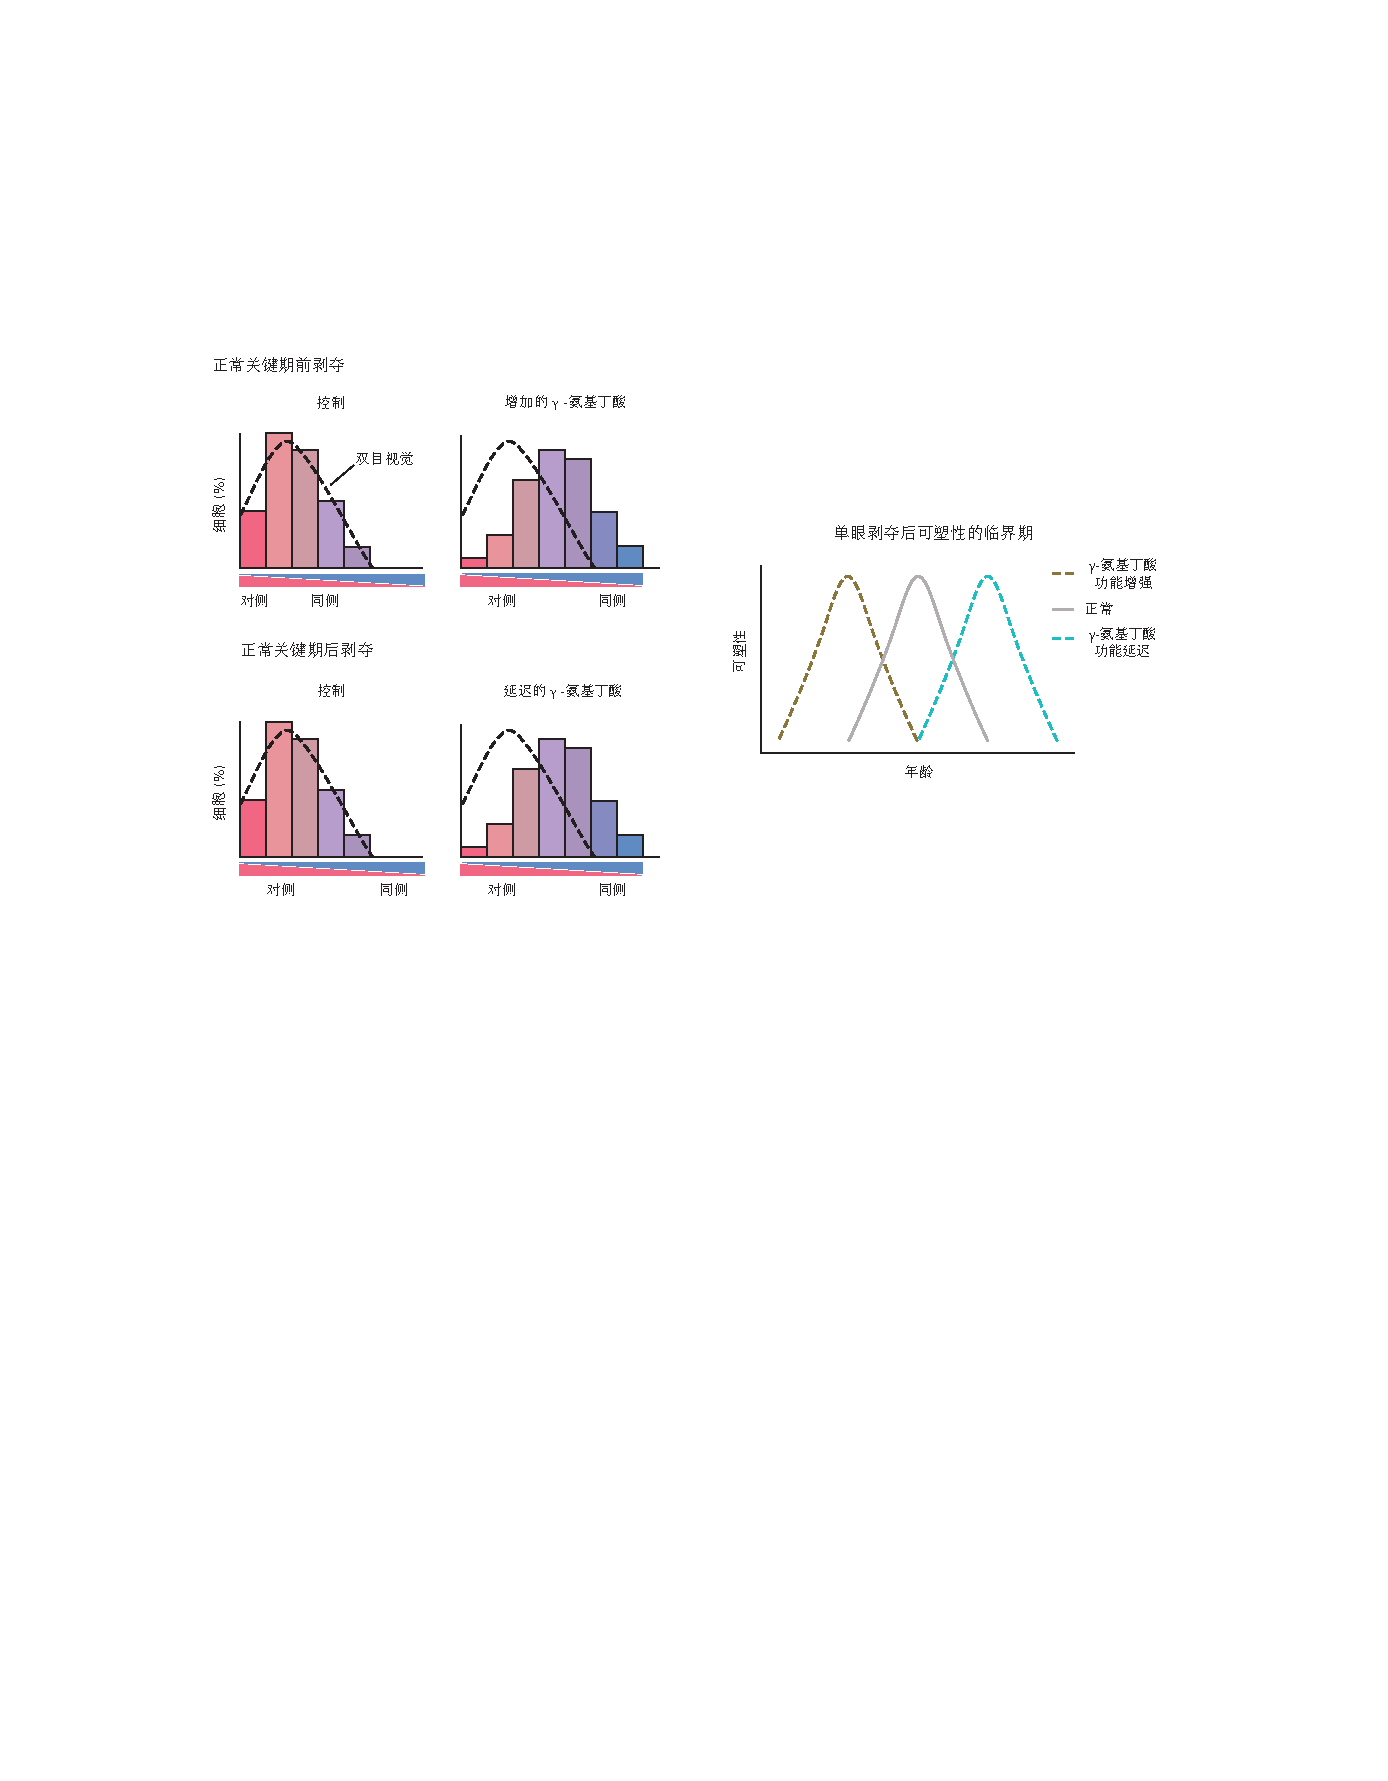
\includegraphics[width=1.0\linewidth]{chap49/fig_49_9}
	\caption{小鼠眼优势可塑性关键期的时间对\textit{$\gamma$-氨基丁酸}能神经传递水平敏感。
		改变\textit{$\gamma$-氨基丁酸}合成和信号传导的状态会改变单眼剥夺可以改变视觉皮层神经元反应特性的时期。
		增强\textit{$\gamma$-氨基丁酸}信号(通过使用苯二氮卓类药物)可将单眼剥夺的关键时期提前至发育期。
		相比之下,延迟\textit{$\gamma$-氨基丁酸}信号(通过基因减少\textit{$\gamma$-氨基丁酸}合成,然后在稍后时间施用苯二氮卓类药物)将单眼剥夺的关键时期转移到较晚的发育时期\cite{daw1998critical}。}
	\label{fig:49_9}
\end{figure}



\subsection{突触结构在关键时期发生改变}

许多研究都在寻找与视觉皮层对闭眼和睁眼输入的反应性改变相关的结构变化。
特别注意树突棘作为可塑性的潜在位点。


棘是许多皮层神经元树突的小突起,其上形成兴奋性突触。
它们是动态结构,它们的出现和消失被认为反映了突触的形成和消除。
脊柱运动在出生后早期发育过程中尤为明显,脊柱动力学和数量的增加与行为变化有关。


在一只眼睛闭合后,观察到小鼠视觉皮层神经元的运动性和树突棘数量发生显著变化。
幼鼠闭眼两天后,视觉皮层神经元上树突棘的运动和转换增加,表明突触连接开始重新排列(图~\ref{fig:49_10})。
几天后,刺的数量开始发生变化;
锥体神经元顶端树突上的刺数最初减少,但在较长时间的剥夺后再次增加。


\begin{figure}[htbp]
	\centering
	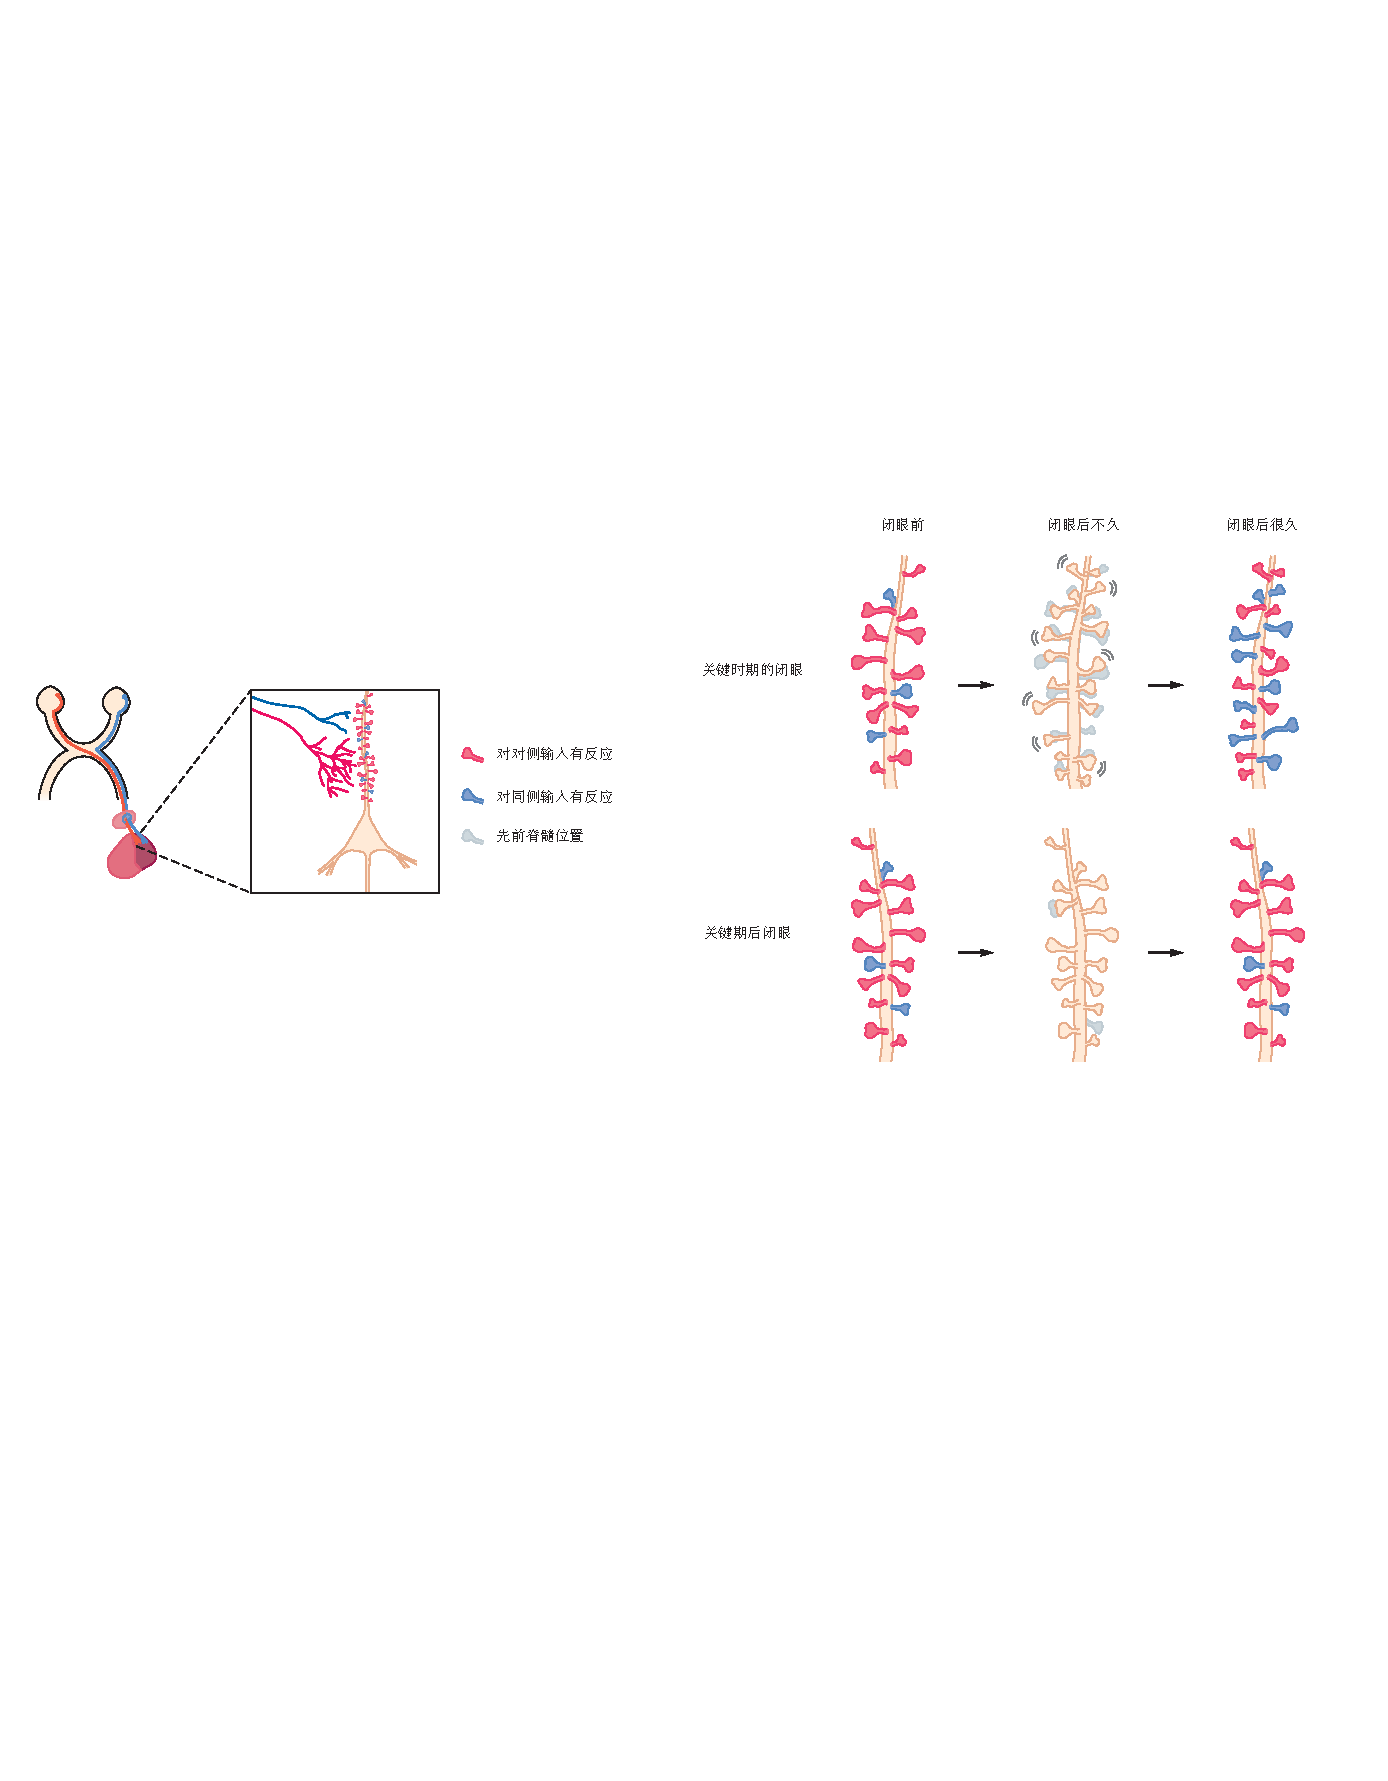
\includegraphics[width=1.0\linewidth]{chap49/fig_49_10}
	\caption{一只眼睛闭上后,小鼠视觉皮层中树突棘的运动会发生变化。
		视觉皮层中锥体神经元的树突有许多棘,其密度在正常情况下保持相对恒定。
		在双眼发育的关键时期闭上一只眼睛(在本例中为对侧)会增强树突棘的运动性,并且随着时间的推移,会导致从睁开的眼睛接收突触输入的棘的比例增加。
		如果在关键期后闭上眼睛,则不会观察到脊柱运动的类似变化\cite{oray2004dendritic}。}
	\label{fig:49_10}
\end{figure}


脊柱运动和数量的这些变化可以与关键期的三个已知特征相关联。
首先,这些变化主要发生在双眼细胞所在的皮层表层和深层,而不是发生在第 IV 层。
其次,它们只出现在正常接收双眼输入的视觉皮层部分。
第三,它们在成年小鼠闭眼后不会发生(图~\ref{fig:49_10})。


总之,这些结果支持脊柱动力学与关键时期可塑性的联系。
根据一个模型,脊柱运动可能是由于睁眼和闭眼输入双眼神经元的不平衡造成的,它可能反映了突触重排的第一阶段。
反过来,脊柱的丢失,可能还有突触的丢失,在时间和空间上对应于闭眼输入的丢失,并可能为这种丢失的持久性提供结构基础。
新刺的后期生长发生在对睁眼的反应增加时或之后,并且可能是适应性重排的基础,这种重排允许皮层充分利用可用的输入。



\subsection{丘脑输入在关键时期被重塑}

如图~\ref{fig:49_4}~所示,脊柱的局部变化与眼优势柱的大规模结构变化有何关系?
当从外侧膝状体核发育的轴突首先到达皮层时,几个神经元的末端广泛重叠。
每根纤维在视觉皮层的一个区域上延伸几个分支,该区域跨越几个未来的眼优势列。
随着皮层的成熟,轴突收缩一些分支,扩展其他分支,甚至形成新的分支(图~\ref{fig:49_11}A)。


\begin{figure}[htbp]
	\centering
	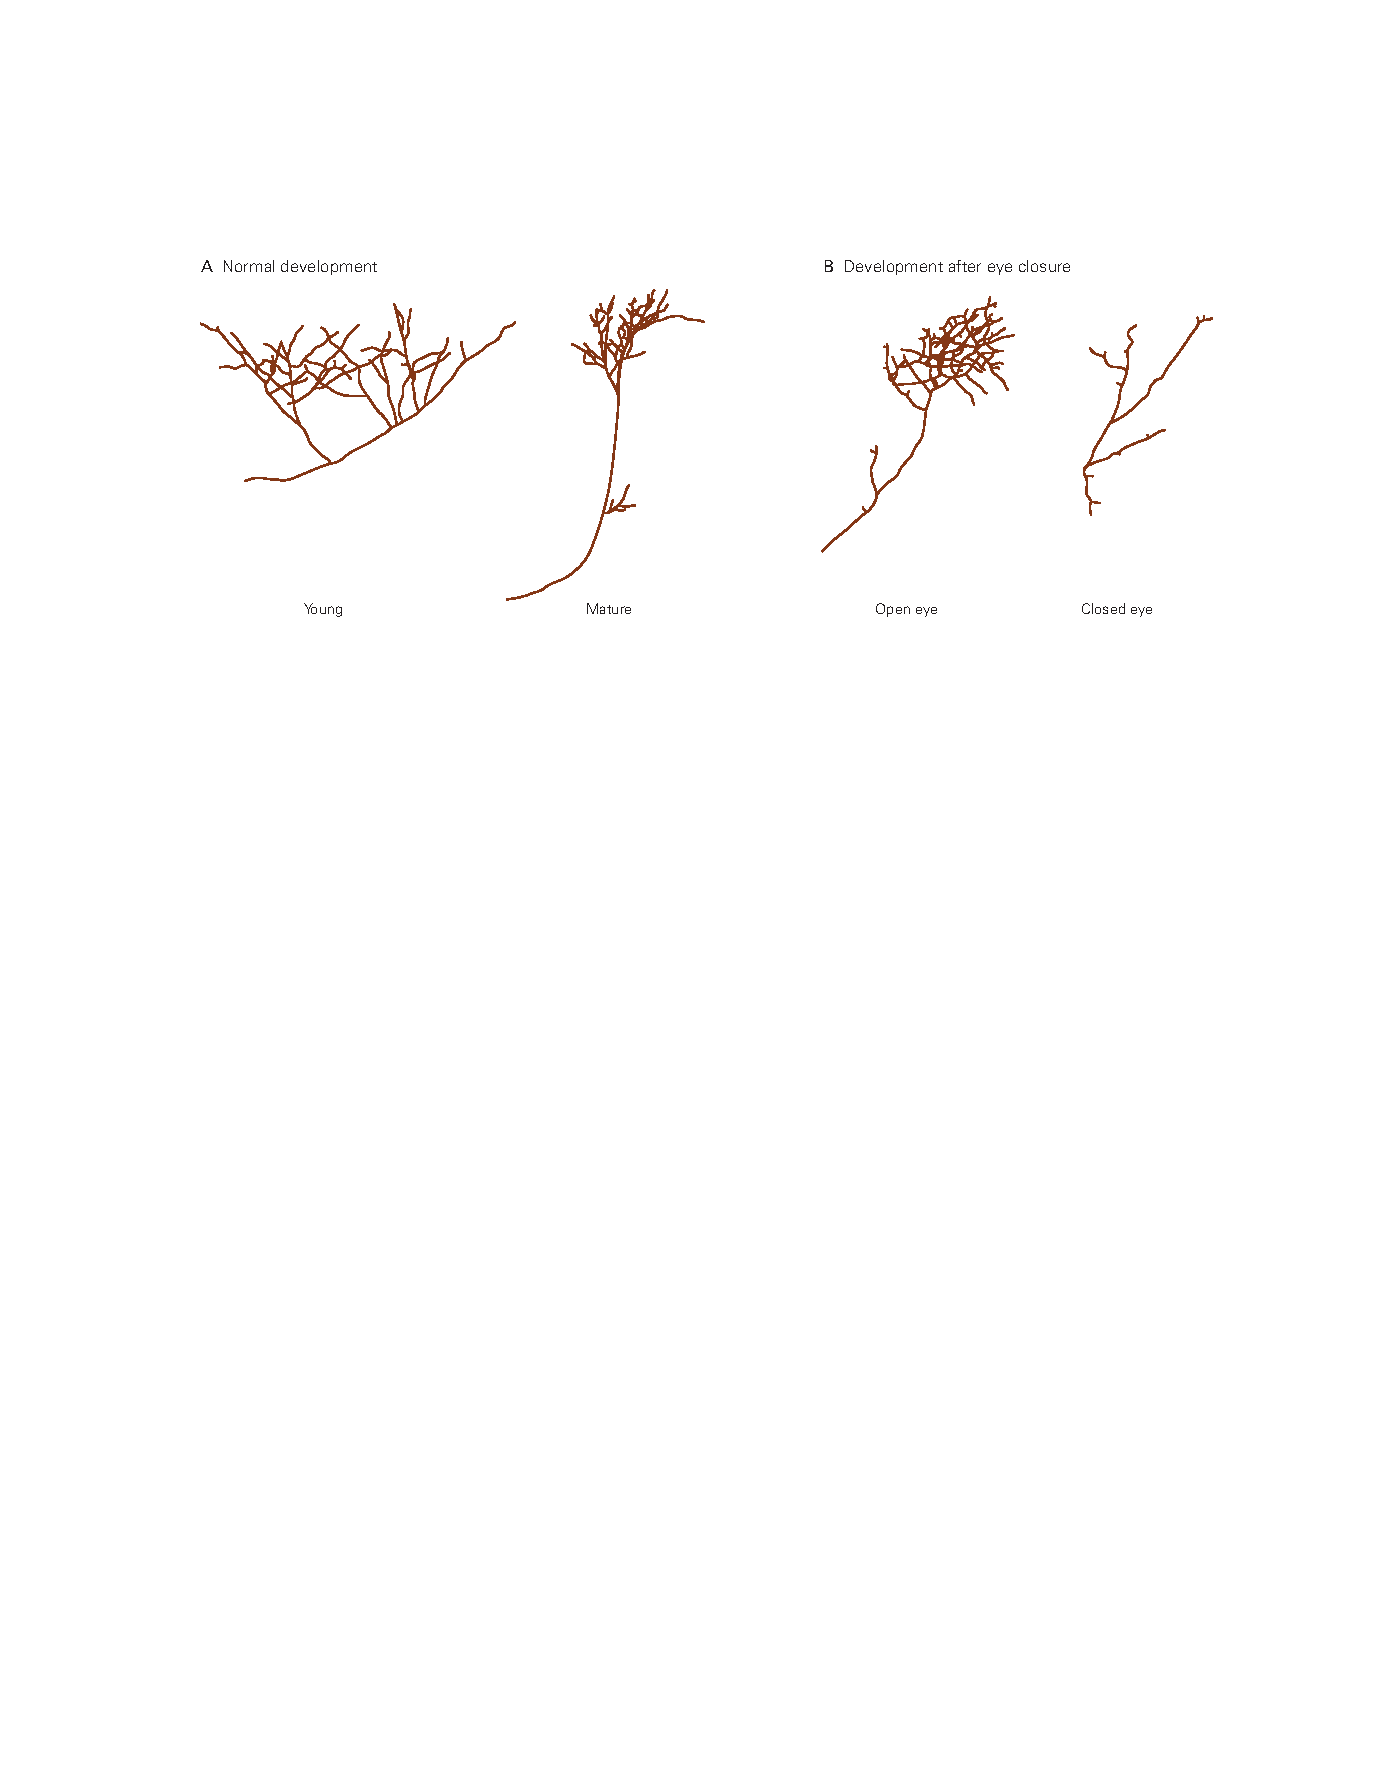
\includegraphics[width=1.0\linewidth]{chap49/fig_49_11}
	\caption{小猫视觉皮层中丘脑皮层纤维的分支在闭眼后发生变化\cite{antonini1993rapid}。
		\textbf{A.} 在正常的出生后发育过程中,外侧膝状体核细胞的轴突在视觉皮层中广泛分支。
		分支最终会局限于一个小区域。
		\textbf{B.} 一只眼睛闭上后,与睁开的眼睛相比,来自那只眼睛的通路中的神经元末梢明显更小。}
	\label{fig:49_11}
\end{figure}


随着时间的推移,每个膝状体神经元几乎完全连接到单个列中的一组相邻皮层神经元。
通过某些轴突的修剪或收缩以及其他轴突的萌芽,乔木被隔离成柱状。
这种轴突收缩和发芽的双重过程在发育过程中广泛发生在整个神经系统中。


一只眼睛闭上后会发生什么?
闭眼的轴突处于劣势,并且比正常比例更大的轴突缩回。
同时,来自睁眼的轴突在被纤维空出的位点发芽新的末端,否则这些纤维会从闭眼传递输入(图~\ref{fig:49_11}B)。
如果动物在轴突分离的关键时期早期被剥夺了使用一只眼睛的权利,轴突收缩和生长的正常过程就会受到干扰。
相比之下,如果动物在眼优势柱几乎完全分离后被剥夺了使用一只眼睛的权利,那么从睁开的眼睛传递输入的轴突实际上会在它们早些时候腾出的皮层区域发芽侧枝(见图~\ref{fig:49_5})。


最初,人们认为单眼剥夺动物的丘脑皮层轴突重排导致皮层对睁眼和闭眼的反应发生变化。
我们现在知道,通过脊柱的电生理记录和成像,生理变化和突触改变先于大规模的轴突重排。
因此,轴突重塑可能有助于使这些变化持久且不可逆转,而不是引起生理变化。
那么问题就变成了:大脑皮层内突触结构和功能的改变如何导致输入的改变?


一种想法是突触活动调节皮层神经元的神经营养因子的分泌。
然后,这些因素可能会以牺牲其他神经元为代价来调节某些神经元的存活(第~\ref{chap:chap46}~章),或者以牺牲其他神经元为代价促进某些轴突乔木的扩张。
其中一个因素,\textit{脑源性神经营养因子}由皮层神经元合成和分泌,施用过量的\textit{脑源性神经营养因子}或干扰其受体 \textit{酪氨酸激酶}B 会改变眼优势柱的形成。
然而,解释\textit{脑源性神经营养因子}的作用并不简单。
\textit{脑源性神经营养因子}和 \textit{酪氨酸激酶}B 信号以多种方式影响皮层,包括促进丘脑皮层轴突的生长。
\textit{脑源性神经营养因子}还可以加速抑制回路的成熟,如上所述,抑制回路可以影响可塑性。
目前尚不清楚\textit{脑源性神经营养因子}是否是优先促进某些乔木扩张的竞争的特定催化剂。



\subsection{突触稳定有助于结束关键期}

关键时期的一个标志是经验影响神经回路发展的时间间隔是有限的。 是什么让这段可塑性增强的时期结束了?


由于突触和回路在关键时期不稳定,研究人员一直在寻找可能导致稳定的皮层发育变化。
一个参数是轴突的髓鞘形成状态,它发生在关键期结束前后。
髓磷脂的形成对发芽和轴突生长造成了物理障碍。
此外,如第~\ref{chap:chap50}~章中详细讨论的那样,髓磷脂包含主动抑制轴突生长的因子,例如\textit{勿动蛋白}和髓磷脂相关糖蛋白。 
在缺乏\textit{勿动蛋白}或其受体之一\textit{勿动蛋白受体}的突变小鼠中,关键期一直开放到成年期,这表明这些受体的出现通常有助于关闭关键期(图~\ref{fig:49_12})。


\begin{figure}[htbp]
	\centering
	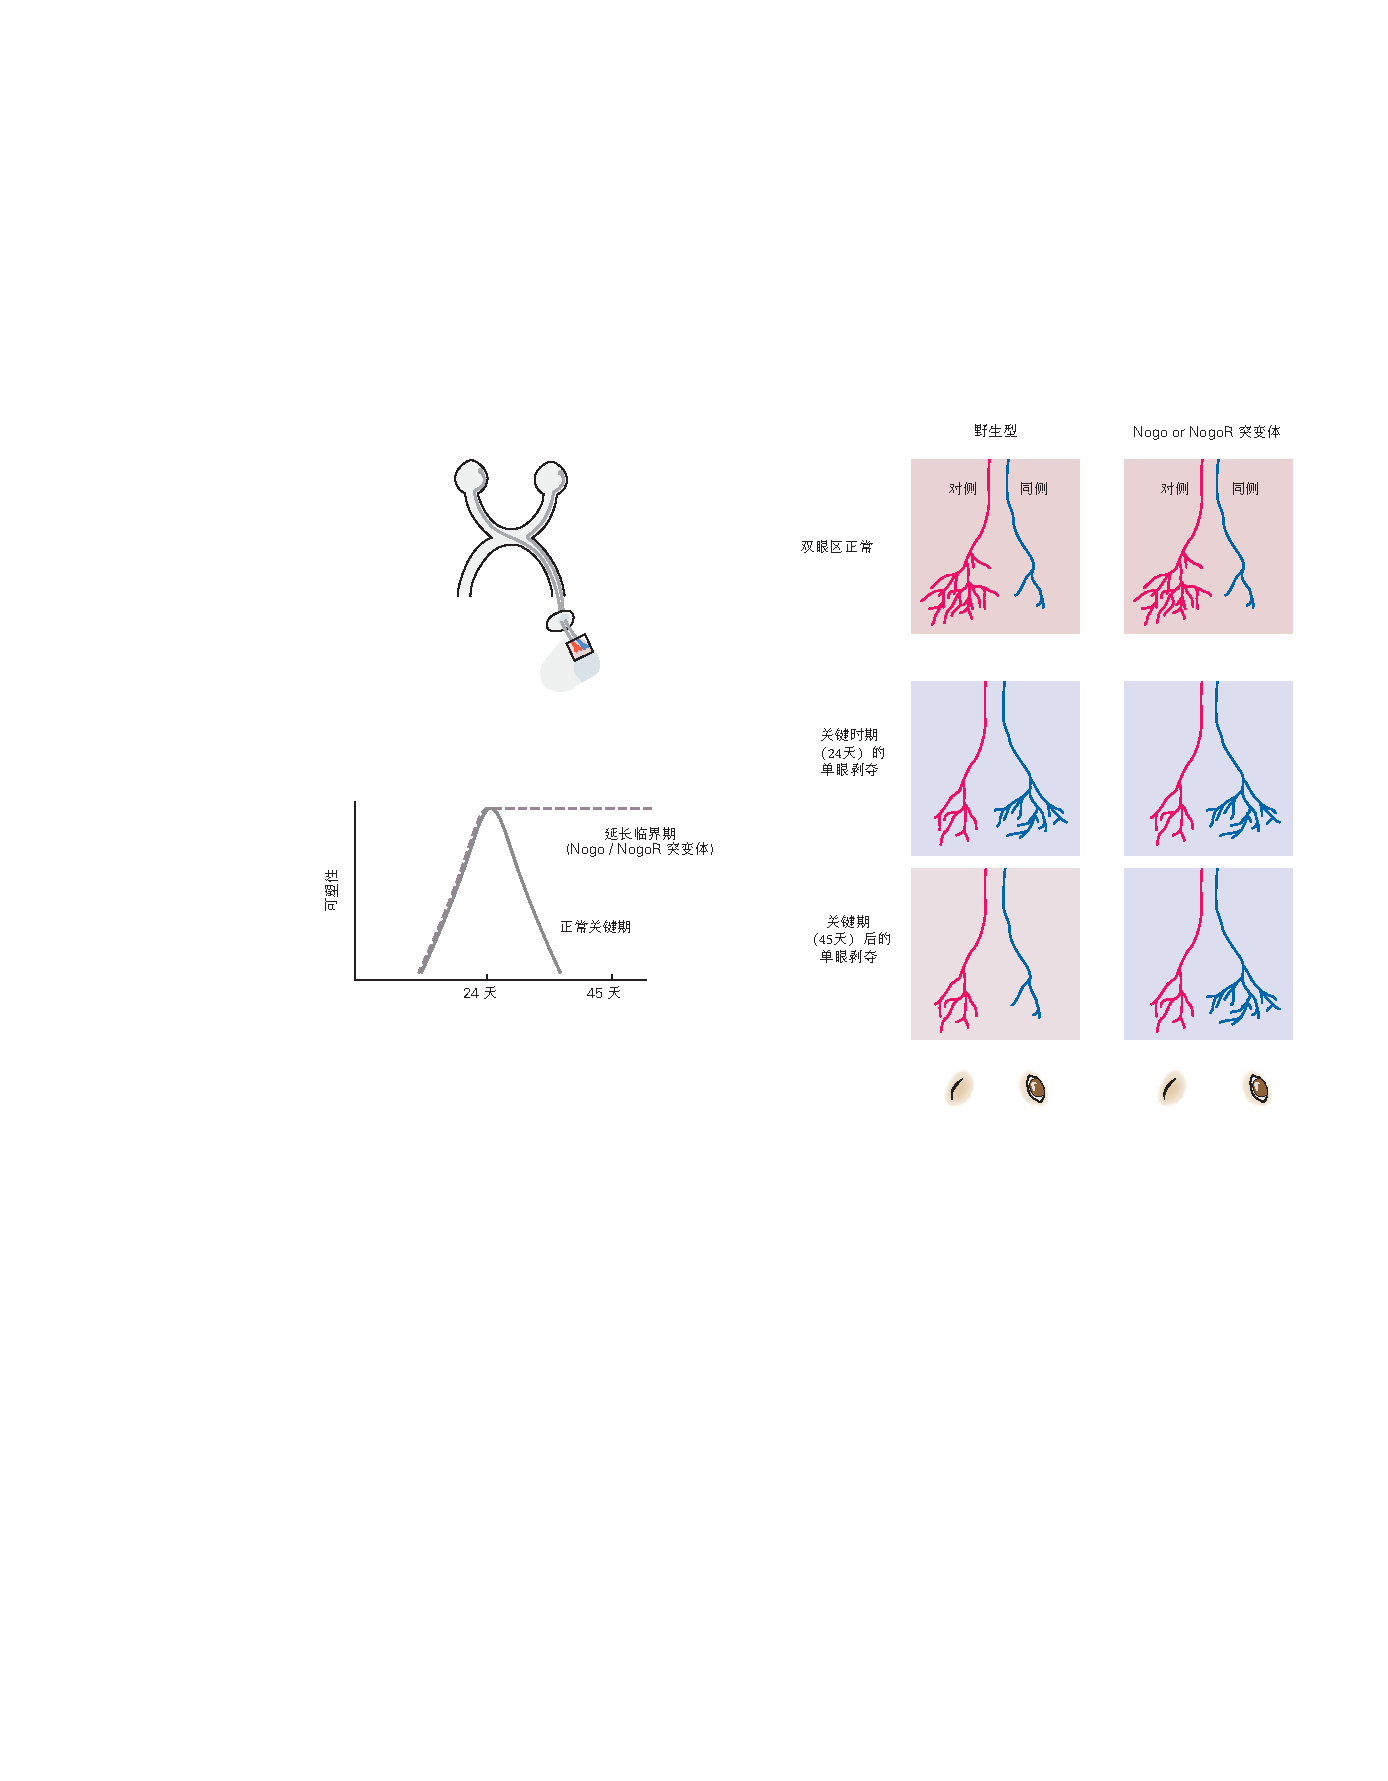
\includegraphics[width=1.0\linewidth]{chap49/fig_49_12}
	\caption{在缺乏\textit{勿动蛋白}信号的小鼠中,单眼剥夺的关键期会延长。
		这些图显示了丘脑皮层轴突的树枝化模式,这些轴突将信号从对侧和同侧眼睛传送到视觉皮层的双眼区。
		关键时期的单眼剥夺导致野生型小鼠和\textit{勿动蛋白}或\textit{勿动蛋白}受体突变体小鼠双眼区神经元的眼睛偏好发生变化。
		在正常的关键期(45 天)之后,在具有突变型\textit{勿动蛋白}-A 或\textit{勿动蛋白}受体的小鼠中,眼睛偏好的变化仍在继续,但在野生型小鼠中则没有。
		该图显示消除\textit{勿动蛋白}信号可防止关键期结束\cite{mcgee2005experience}。}
	\label{fig:49_12}
\end{figure}


另一种可能的闭合剂是神经元网,一种包裹某些类别抑制性神经元的糖胺聚糖网。
这些网在关键期结束时形成。
消化神经周围网的软骨素酶的输注可保持可塑性。
因此,一旦突触生长和重排的分子障碍发挥作用,关键时期可能会结束。


额外的关闭代理可能是神经元固有的。
在第~\ref{chap:chap50}~章中,我们将看到神经元的生长程序随着年龄的增长而减少,在第~\ref{chap:chap51}~章中,我们将描述表观遗传机制,该机制“锁定”在出生后早期建立的基因表达的经验依赖模式。


为什么要结束关键时期?
大脑保持其重塑到成年期的能力不是很有利吗?
或许不是:我们的大脑适应感官输入变化、身体逐渐成长(例如,影响双眼对应的双眼距离的增加)以及各种先天性疾病的能力是一项宝贵的资产。
在极端情况下,如果一只眼睛失去了,将所有可用的皮层空间用于剩余的眼睛是有利的。
然而,如果一只眼睛的视力在成年期因疾病或受伤暂时丧失,人们不希望大规模重组,可能伴随技能和记忆的丧失。
因此,在关键时期增强可塑性可能代表灵活性和稳定性之间的适应性妥协。



\section{独立于经验的自发神经活动导致早期回路完善}

如上所述,在视觉体验开始之前,猫和猴子的视觉皮层就开始分离成眼优势柱。
是什么推动了这个早期的隔离阶段?
一种可能性是来自同侧和对侧眼睛的轴突带有不同的分子标签,导致它们相互关联。
类似的机制发生在嗅觉投射的形成中(第~\ref{chap:chap48}~章)。
然而,在视觉投影中还没有发现这样的分子或机制。
相反,隔离似乎依赖于自发活动,这不仅发生在感官输入之前,而且还表现出惊人的模式。
这种机制最初是在对外侧膝状体的研究中发现的,其神经元为视觉皮层提供视觉输入。


来自两只眼睛的视网膜神经节细胞的乔木被分离到外侧膝状核中的交替层中,就像这个核的投射被分离到视觉皮层中交替的眼优势柱中一样(图~\ref{fig:49_13})。 
在这两种结构中,单个轴突首先在多个域(膝状核中的层,皮层中的柱)中形成末端。
后来,终端通过改进过程被隔离。
改进包括在“合适的”层中生长顶生乔木和从不合适的层中消除顶生乔木(第~\ref{chap:chap48}~章)。


\begin{figure}[htbp]
	\centering
	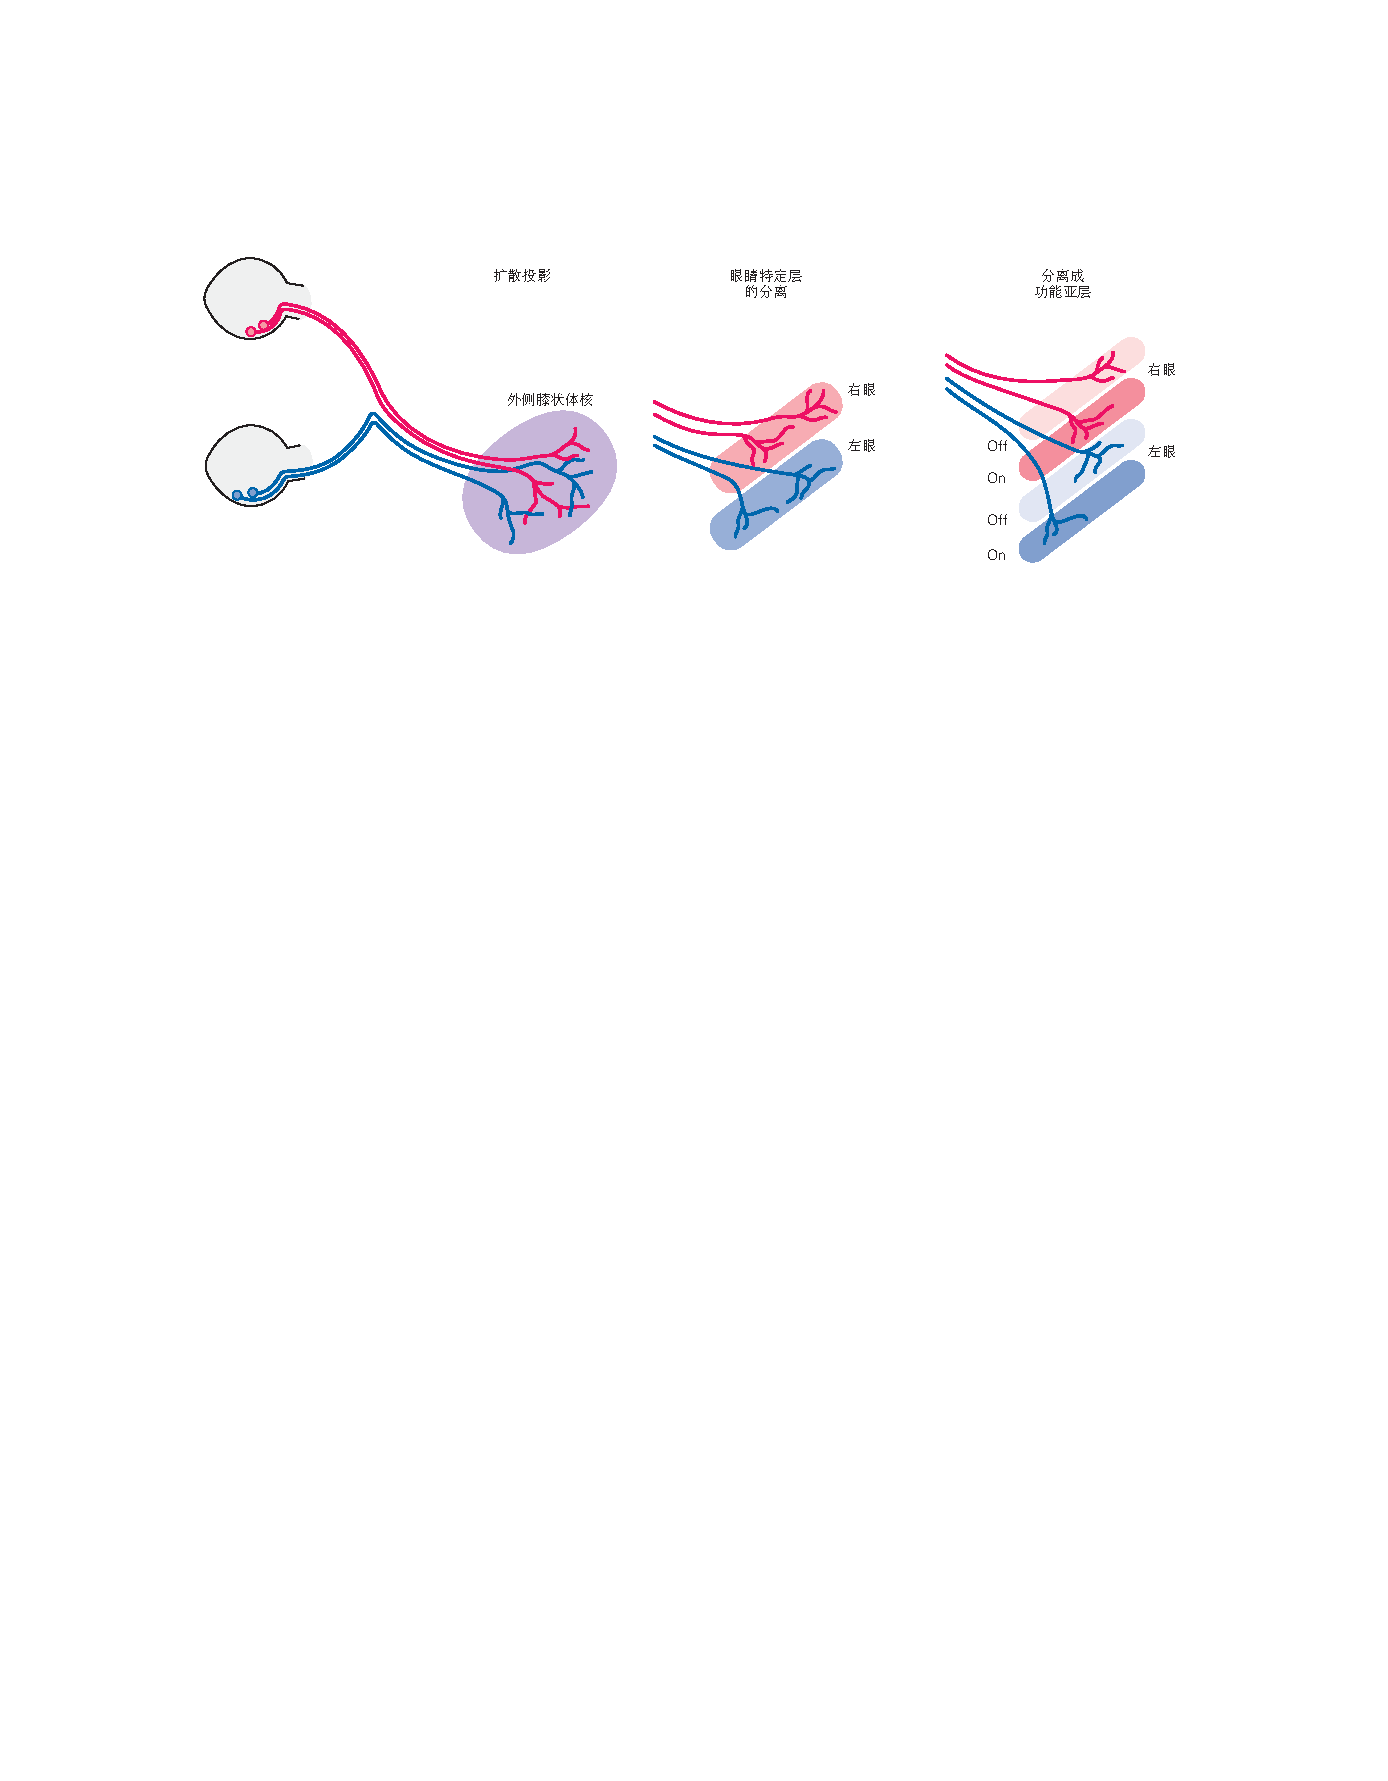
\includegraphics[width=1.0\linewidth]{chap49/fig_49_13}
	\caption{\textit{外侧膝状体核}中的视网膜神经节细胞的末端在正常发育过程中变得分离。
		在发育的早期阶段,每只眼睛的轴突末端混合在一起,但在后期阶段,它们分离到不同的细胞核层中。
		在某些物种中,一只眼睛的轴突甚至分离成功能特化的子层(雪貂的上下层)\cite{sanes1999formation}。}
	\label{fig:49_13}
\end{figure}


与在皮层中一样,将河豚毒素应用于视神经会破坏每只眼睛输入的分离,表明活动对于分离至关重要。
然而,与大脑皮层不同的是,输入的分离在视觉体验开始之前就已完成:在猴子出生之前,在小鼠出生后但在睁眼之前。
因此,视觉不能驱动隔离所必需的神经活动。


事实证明,视网膜神经节神经元的轴突在子宫内自发活跃,远在眼睛睁开之前。
相邻的神经节细胞以持续几秒钟的同步爆发形式发射,然后是可能持续几分钟的静默期。
对整个视网膜上的视网膜神经节神经元的活动进行采样表明,这些爆发以波状方式在大部分视网膜上传播(图~\ref{fig:49_14})。
这种神经节细胞活动模式似乎与来自视网膜上层无长突细胞的兴奋性输入相协调(第~\ref{chap:chap22}~章)。


\begin{figure}[htbp]
	\centering
	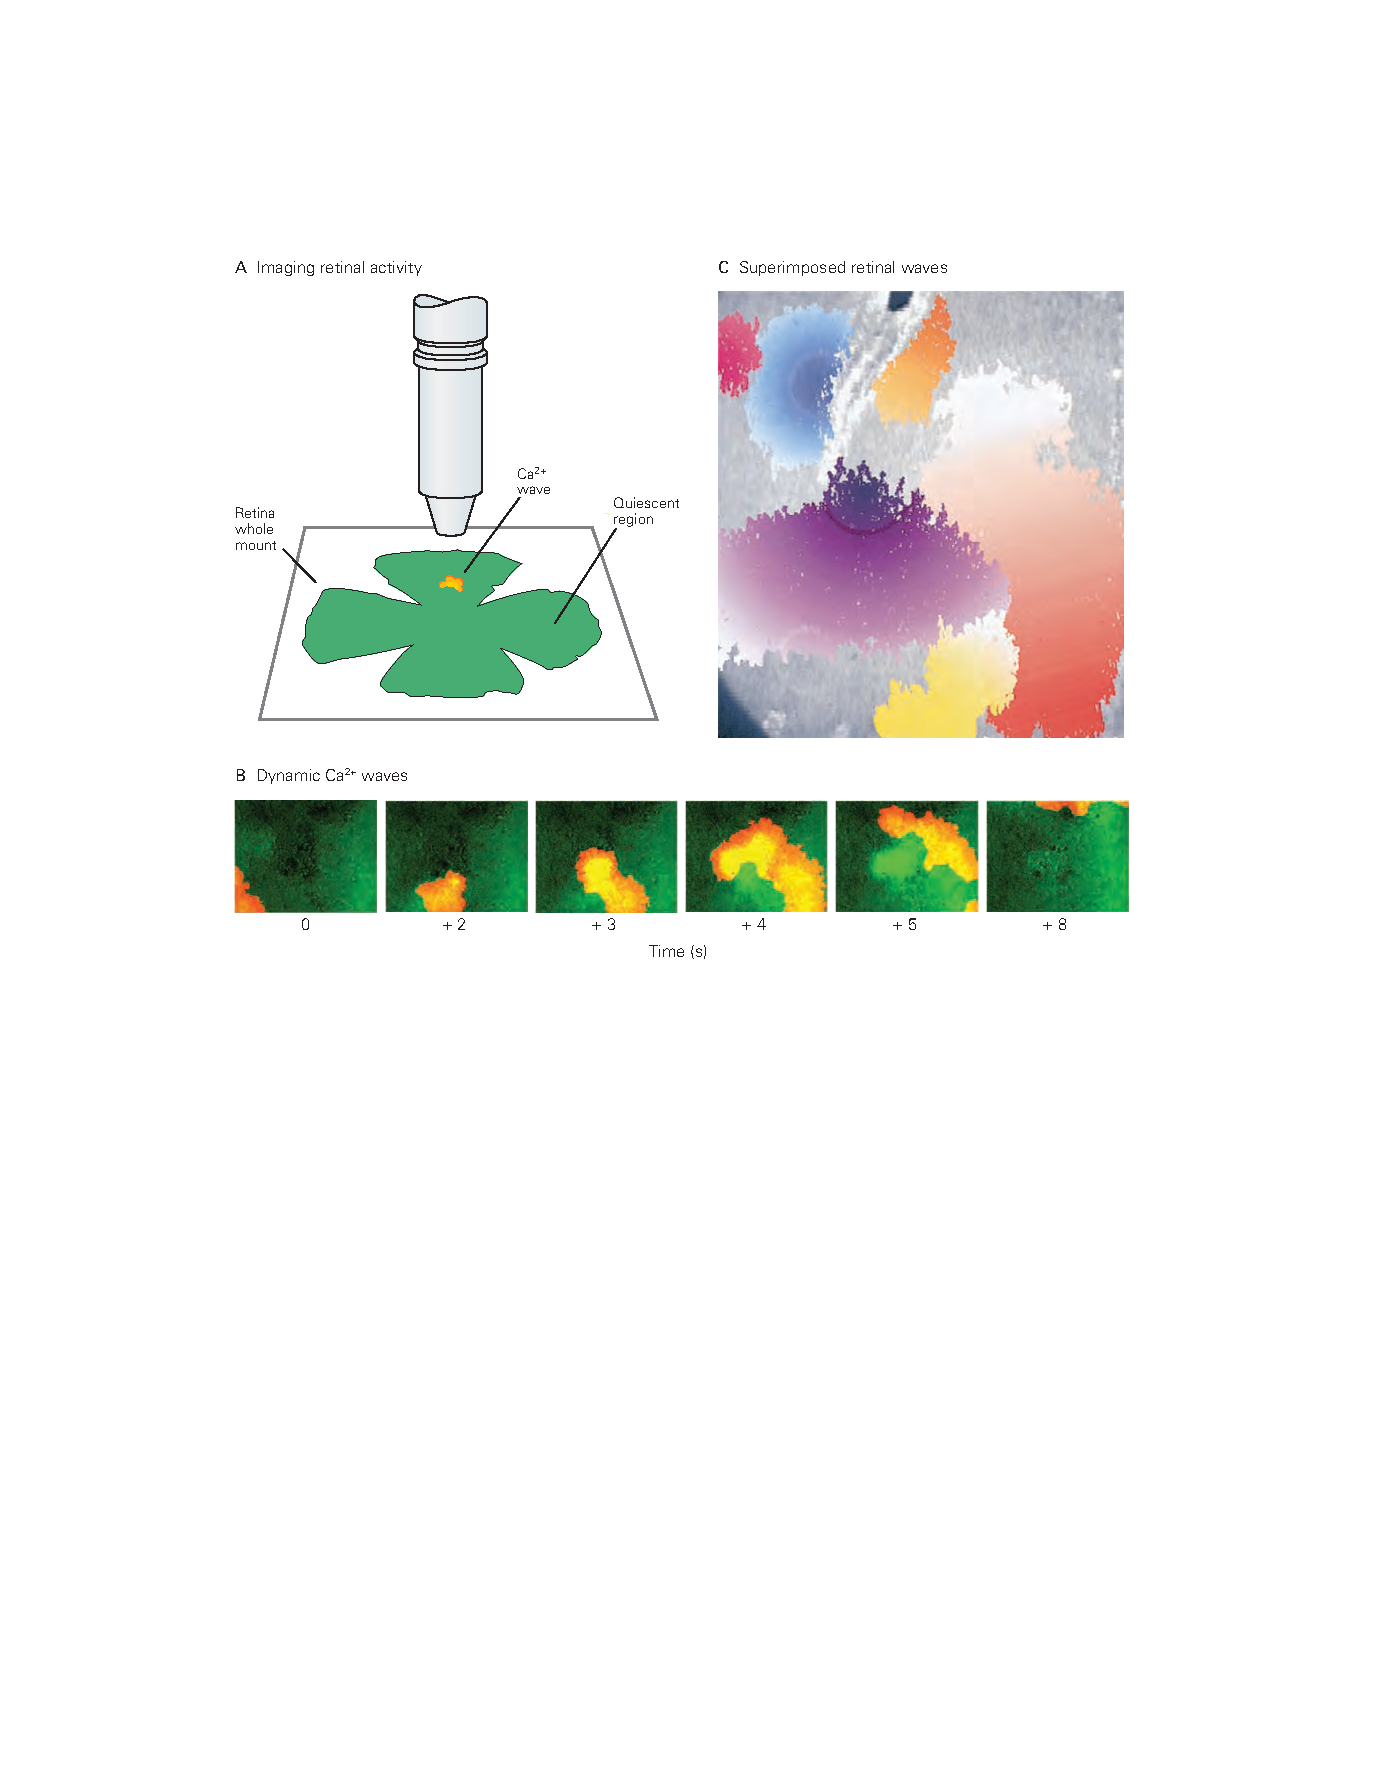
\includegraphics[width=1.0\linewidth]{chap49/fig_49_14}
	\caption{发育中的视网膜中神经活动的相关波。
		\textbf{A.} 哺乳动物视网膜平装标本中视网膜神经节神经元活动的显微观察。
		神经活动的自发波通过监测 \ce{Ca^2+} 瞬变(黄色域)在细胞加载染料后可视化,染料会响应细胞内 \ce{Ca^2+} 浓度的变化而改变其荧光发射光谱。
		\textbf{B.} 这些来自电影序列的静止图像显示了一个 \ce{Ca^2+} 活动焦点(黄色域)在视网膜上的传播。
		相隔 1 秒拍摄图像。
		活动焦点内的许多细胞被同步激活。
		\textbf{C.} 此图像中叠加了随时间记录的视网膜活动波。
		离散波以不同颜色表示;
		波的起源由较暗的色调表示。
		这些波起源于不同的视网膜病灶,并向不同的、不可预测的方向传播。}
	\label{fig:49_14}
\end{figure}


一组选定的神经节神经元的自发同步放电会激发外侧膝状体核中的一组局部神经元。
这种同步活动似乎以牺牲其他附近的突触为代价来加强这些突触,这可能是通过类似于为依赖于经验的改进而假设的赫布机制。
这并不意味着视觉诱发的活动在塑造视网膜生成途径中没有作用。
在后期阶段,其他方面的改进,例如突触沿轴突的空间重排,由视觉体验调节。


自发活动可以导致回路细化的发现为视觉皮层输入的初始分离提供了可能的解释。
更一般地说,将依赖于活动的回路细化分为两个阶段,第一个阶段依赖于自发活动,第二个阶段依赖于感觉输入,现在似乎是大脑回路发展的一个普遍主题,在它们有机会对环境刺激作出反应。



\section{依赖于活动的连接细化是大脑回路的一个普遍特征}

我们已经看到,神经活动对于将轴突从两个视网膜分离到外侧膝状核的不同层,然后分离到视觉皮层的不同列至关重要。
活动的这种发展作用是特例,还是活动也会影响视觉系统其他地方甚至大脑其他部分的成熟?
许多系统的研究表明,依赖于活动的细化控制是哺乳动物大脑中神经回路的一般特性。



\subsection{视觉系统开发的许多方面都依赖于活动}

视觉系统中依赖于活动的发育的一个充分研究的例子是视网膜神经节细胞轴突在其中心目标上的地形分布的锐化,这是我们在第~\ref{chap:chap47}~章中介绍的主题。
在脊椎动物中,分子线索(例如肝配蛋白)引导轴突从 视顶盖(在哺乳动物中称为上丘,见图~\ref{fig:47_11})的适当位置,但它们不足以形成精细的视觉图。


组织学和生理学研究发现,最初在上丘/视顶盖中形成的图很粗糙,并且单个视网膜神经节细胞轴突具有大而重叠的轴。
这些轴突乔木后来被修剪成成熟的大小,导致终止区域更加受限和精确。
如果视网膜活动受到抑制,则只会形成最初的粗略地图。


在视觉地图形成中重要的是活动模式还是活动本身?
换句话说,活动仅仅是精化的先决条件,还是它具有组织作用,确切地决定哪些轴突在竞争中获胜或失败?
许多实验表明,后一种想法更接近事实。


在一项研究中,对在仅由频闪灯短暂闪光照明的水箱中饲养的鱼进行了视网膜直立图的准确性评估。
对照组在正常的实验室环境中饲养。
在两种条件下,呈现给鱼的总光强度相似,但产生的模式却大不相同。
在对照鱼中,当鱼在鱼缸周围游动时,图像随意地落在视网膜的各个部位。
这种输入产生了由上述自发活动波产生的那种局部同步活动:相邻的神经节细胞倾向于一起发射,但与远处神经节细胞的发射模式几乎没有相关性。
在这些鱼中,地图变得精确。
相比之下,频闪照明同步激活几乎所有的神经节细胞,在这些鱼中,\textit{连接视网膜和中脑顶盖神经纤维的}地图仍然很粗糙。


据推测,顶盖通过判断哪些轴突同步发射来确定哪些视网膜轴突是邻近的,就像外侧膝状体核或视觉皮层中的活动模式决定哪些轴突携带来自同一只眼睛的信号一样。
然后,通过类似于皮层中的机制,这些信息被用来完善地形图。
当所有轴突同步放电时,顶盖无法确定哪些轴突是相邻的;
细化失败,地图仍然很粗糙。



\subsection{感官模式在关键时期得到协调}

我们对世界的体验是通过综合多种方式的感官输入来塑造的。
例如,无论我们是通过触觉、声音还是视觉来定位物体,我们对物体相对于我们身体位置的心理印象都是一样的。
对于每种模式,信息在相关脑区内以有序的方式映射,很像视顶盖和视觉皮层中的\textit{视网膜脑图}。
多模态本地化要求将这些在开发过程中独立形成的地图进行注册。
这方面的细化发生在关键时期。


对谷仓猫头鹰的研究提供了在关键时期如何协调听觉和视觉地图的见解。
白天,猫头鹰使用视觉来定位它们的猎物(老鼠或其他小型啮齿动物),但在晚上,它们依靠听觉线索,而在黄昏时,两个感觉通道都会被使用。
如果猫头鹰要成功找到猎物,声音的定位就必须精确,直观上显而易见的是,同一位置的视觉和听觉线索需要保持一致。


与人类一样,猫头鹰的听觉定位是由神经元的存在引起的,这些神经元对两只耳朵感知到的声音的敏感度不同。 例如,从左侧声源发出的声音到达左耳的时间比到达右耳的时间稍快,而且在左耳的声音稍大。
这些差异帮助我们确定水平空间中声音的发源点(第~\ref{chap:chap28}~章)。
计算声音到达两只耳朵的时间差异尤为重要。
正如基于声速和头部宽度的计算所预期的那样,差异只有几十微秒。
值得注意的是,听觉系统对这些极短的\textit{双耳时间差}很敏感,并且可以从中计算出猎物的位置(图~\ref{fig:49_15})。
此外,视顶盖中许多具有以特定位置为中心的感受野的听觉神经元也被调谐到与空间中同一点发出的声音相对应的\textit{双耳时间差}。
注册在早期阶段不精确,但由于动物的经验,在青春期早期逐渐变得更加精确。


\begin{figure}[htbp]
	\centering
	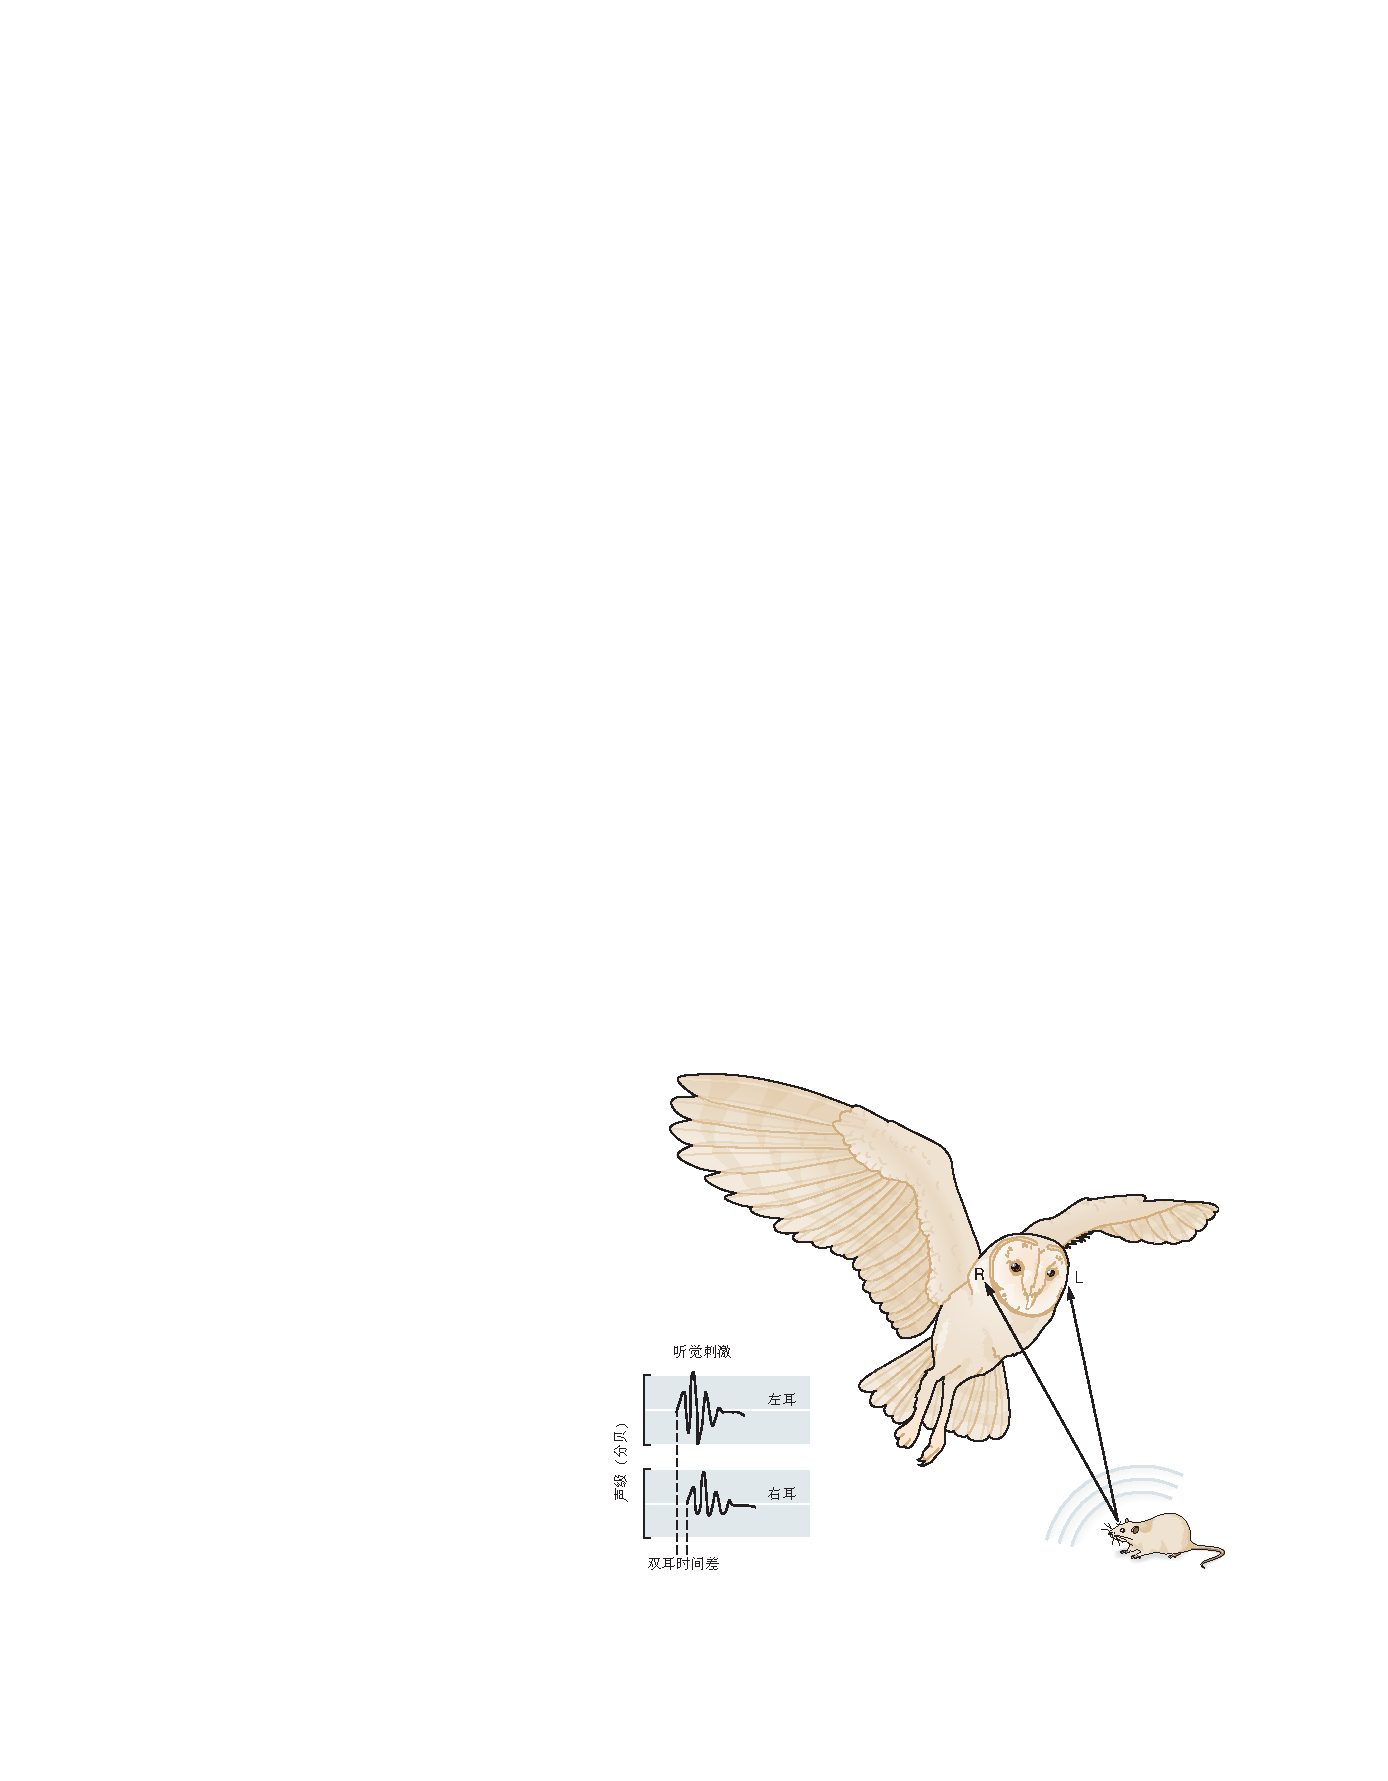
\includegraphics[width=0.78\linewidth]{chap49/fig_49_15}
	\caption{谷仓猫头鹰利用双耳时间差来定位猎物。
		老鼠移动产生的声波被猫头鹰的左耳和右耳接收。
		当猎物发出噪音时,听觉刺激到达两只耳朵的时间差(\textit{双耳时间差})被用来计算猎物目标的精确位置。}
	\label{fig:49_15}
\end{figure}


对这种配准如何发生的关键洞察来自实验,在这些实验中,棱镜安装在年幼猫头鹰的眼睛上。
棱镜水平移动了视网膜图像,因此顶盖中的视觉地图反映了一个系统地偏离其“实际”方向的世界。
这种变化突然破坏了视觉和听觉感受野之间的对应关系。 
然而,在接下来的几周内,顶盖神经元最佳响应的
\textit{双耳时间差},即它们的听觉感受野,发生了变化,直到视觉和听觉映射重新进入记录(图~\ref{fig:49_16})。 
因此,视觉地图指导听觉地图。


\begin{figure}[htbp]
	\centering
	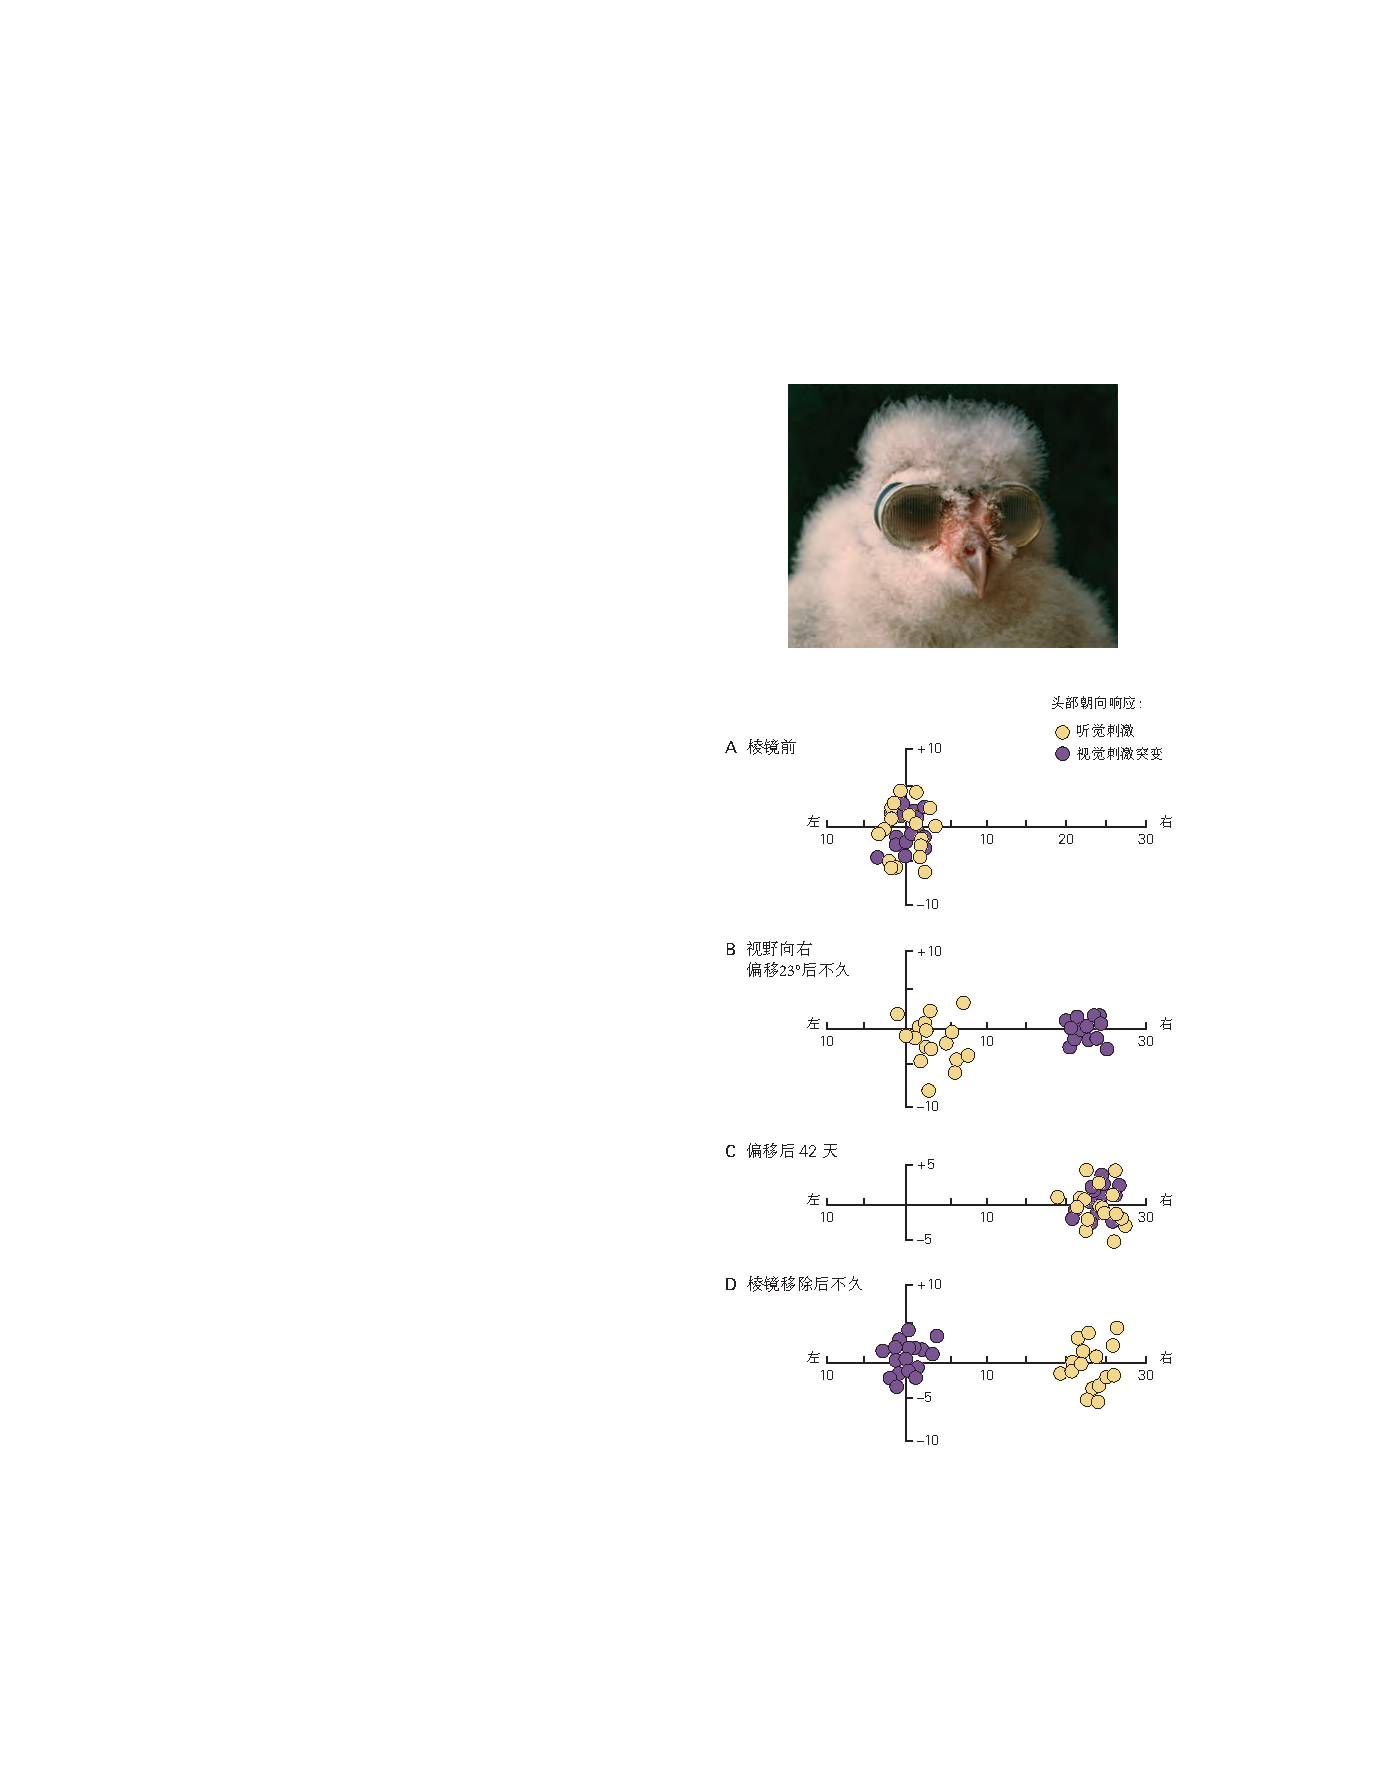
\includegraphics[width=0.59\linewidth]{chap49/fig_49_16}
	\caption{视网膜图像系统位移后猫头鹰视顶盖感觉图的重组。
		青春期猫头鹰的视网膜图像可以被棱镜护目镜移位,将图像从 5° 移动到 30°\cite{knudsen2002instructed}。
		\textbf{A.} 在应用棱镜之前,视觉和听觉神经映射重合。
		\textbf{B.} 棱镜护目镜将视网膜图像位移 23°。
		因此,神经图和听觉图不对齐。
		\textbf{C.} 应用棱镜 42 天后,两张脑图再次一致,因为听觉图已经移动,与视觉图重新对齐。
		\textbf{D.} 棱镜被移除后不久,视觉地图恢复到原来的位置,但听觉地图仍然在其移动的位置。}
	\label{fig:49_16}
\end{figure}


对这种配准如何发生的关键洞察来自实验,在这些实验中,棱镜安装在年幼猫头鹰的眼睛上。
棱镜水平移动了视网膜图像,因此顶盖中的视觉地图反映了一个系统地偏离其“实际”方向的世界。
这种变化突然破坏了视觉和听觉感受野之间的对应关系。
然而,在接下来的几周内,顶盖神经元最佳响应的\textit{双耳时间差},即它们的听觉感受野,发生了变化,直到视觉和听觉映射重新进入记录(图~\ref{fig:49_16})。
因此,视觉地图指导听觉地图。



\subsection{不同的功能和脑区有不同的发展关键期}

并不是所有的大脑回路都会同时稳定下来。
即使在视觉皮层内,组织输入的关键时期在小鼠和猴子的各层之间也不同。
例如,猴子 2 个月大时,视觉皮层\textit{岛前庭皮层}层的神经连接不受单眼剥夺的影响。
相比之下,上层和下层的连接在出生后的几乎整个第一年都继续受到感官体验(或缺乏感官体验)的影响。
视觉系统其他功能的关键时期,例如方向调整,出现在不同的发育阶段(图~\ref{fig:49_18}A)。


\begin{figure}[htbp]
	\centering
	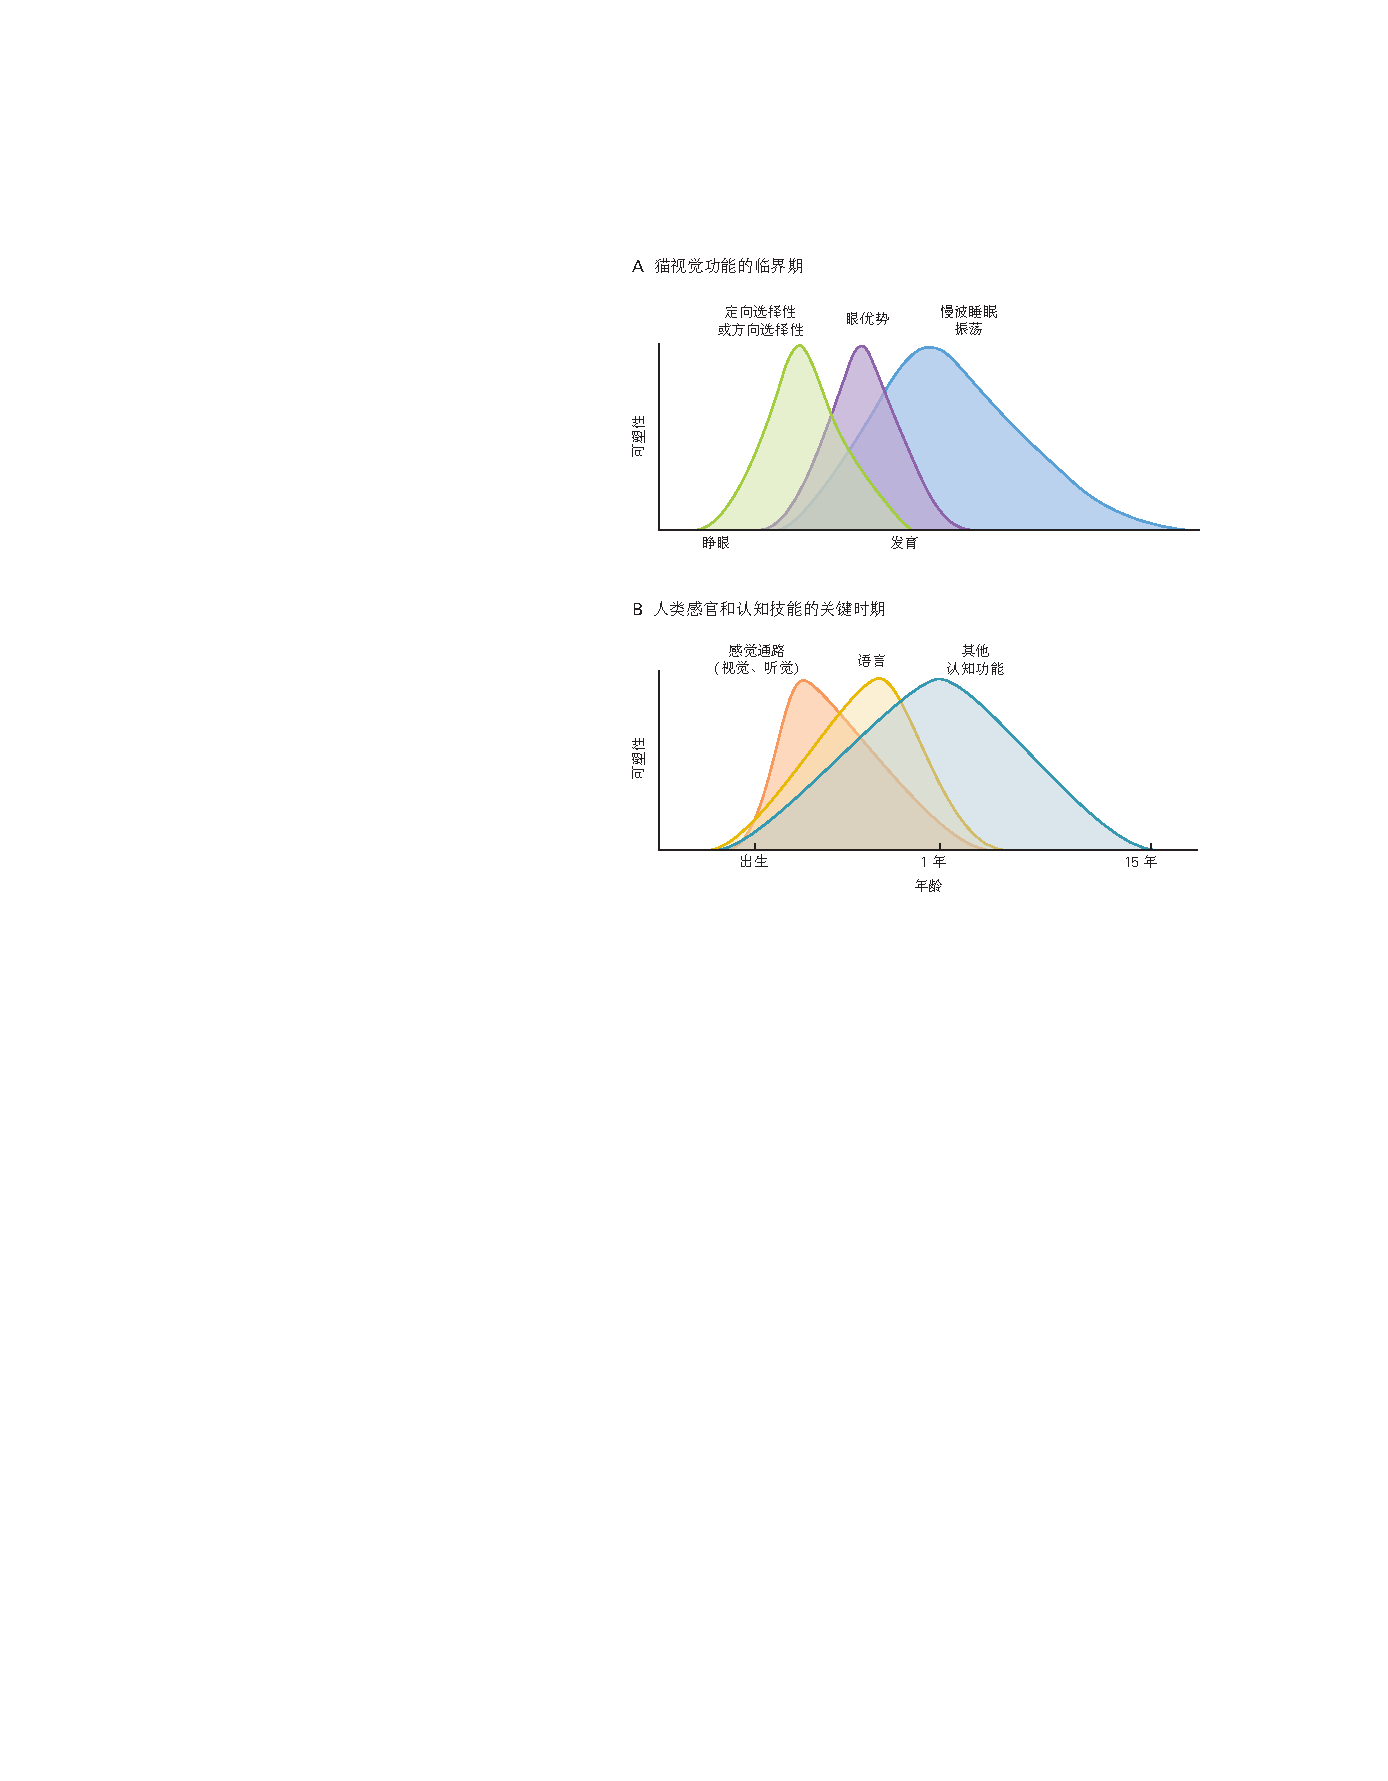
\includegraphics[width=0.69\linewidth]{chap49/fig_49_18}
	\caption{关键期的时间因大脑功能而异。
		\textbf{A.} 在猫中,视觉神经元定向或方向选择性发展的关键时期早于眼优势和慢波睡眠振荡建立的关键时期。 \textbf{B.} 在人类中,感觉处理、语言和认知功能发展的时期各不相同。}
	\label{fig:49_18}
\end{figure}


关键时期的时间也因大脑区域而异(图~\ref{fig:49_18}B)。
感觉剥夺对大脑主要感觉区域的不良后果通常在出生后发育早期就已充分意识到。
相比之下,社会经验可以在更长的时间内影响皮层内连接。
这些差异可以解释为什么某些类型的学习在特定的发展阶段是最佳的。
例如,某些认知能力(语言、音乐和数学)如果要得到发展,通常必须在青春期之前就获得。
此外,在出生后特定的早期阶段对大脑的伤害可能会选择性地影响某些感知能力和行为的发展。



\section{关键时期可以在成年期重新开启}

根据定义,关键时期是有时间限制的。
然而,它们的定义不如原先想象的那么明确。
延长或重新开放成年期的关键时期可以增加大脑的可塑性,并有可能促进从中风和其他损害神经系统离散区域的损伤中恢复。


成人皮层可塑性的一些初步证据来自\textit{梅策尼希}及其同事对体感皮层中猴子手指表征的研究。
正常成年动物神经元感受野的记录表明,每个数字都以有序的方式映射到皮层表面,对不同数字做出反应的区域之间突然不连续(图~\ref{fig:49_19}A)。
一个手指的截肢使该手指的皮层表征最初没有反应,但几个月后,服务于相邻手指的区域填补了空隙(图~\ref{fig:49_19}B)。
就像单眼剥夺后视觉皮层发生的情况一样,体感地图被重新调整,以便皮层可以将其大部分资源用于有用的输入。 相反,当两个手指缝合在一起时,它们接收到一致的输入,两个手指区域边界两侧的皮层带最终对两个区域都有反应(图~\ref{fig:49_19}C)。
这一结果表明,与视觉系统一样,边界可能来自竞争,并且当竞争下降时边界会变得模糊。
最令人惊讶的是,这些影响发生在成年期,在所有已知的关键期结束很久之后。


\begin{figure}[htbp]
	\centering
	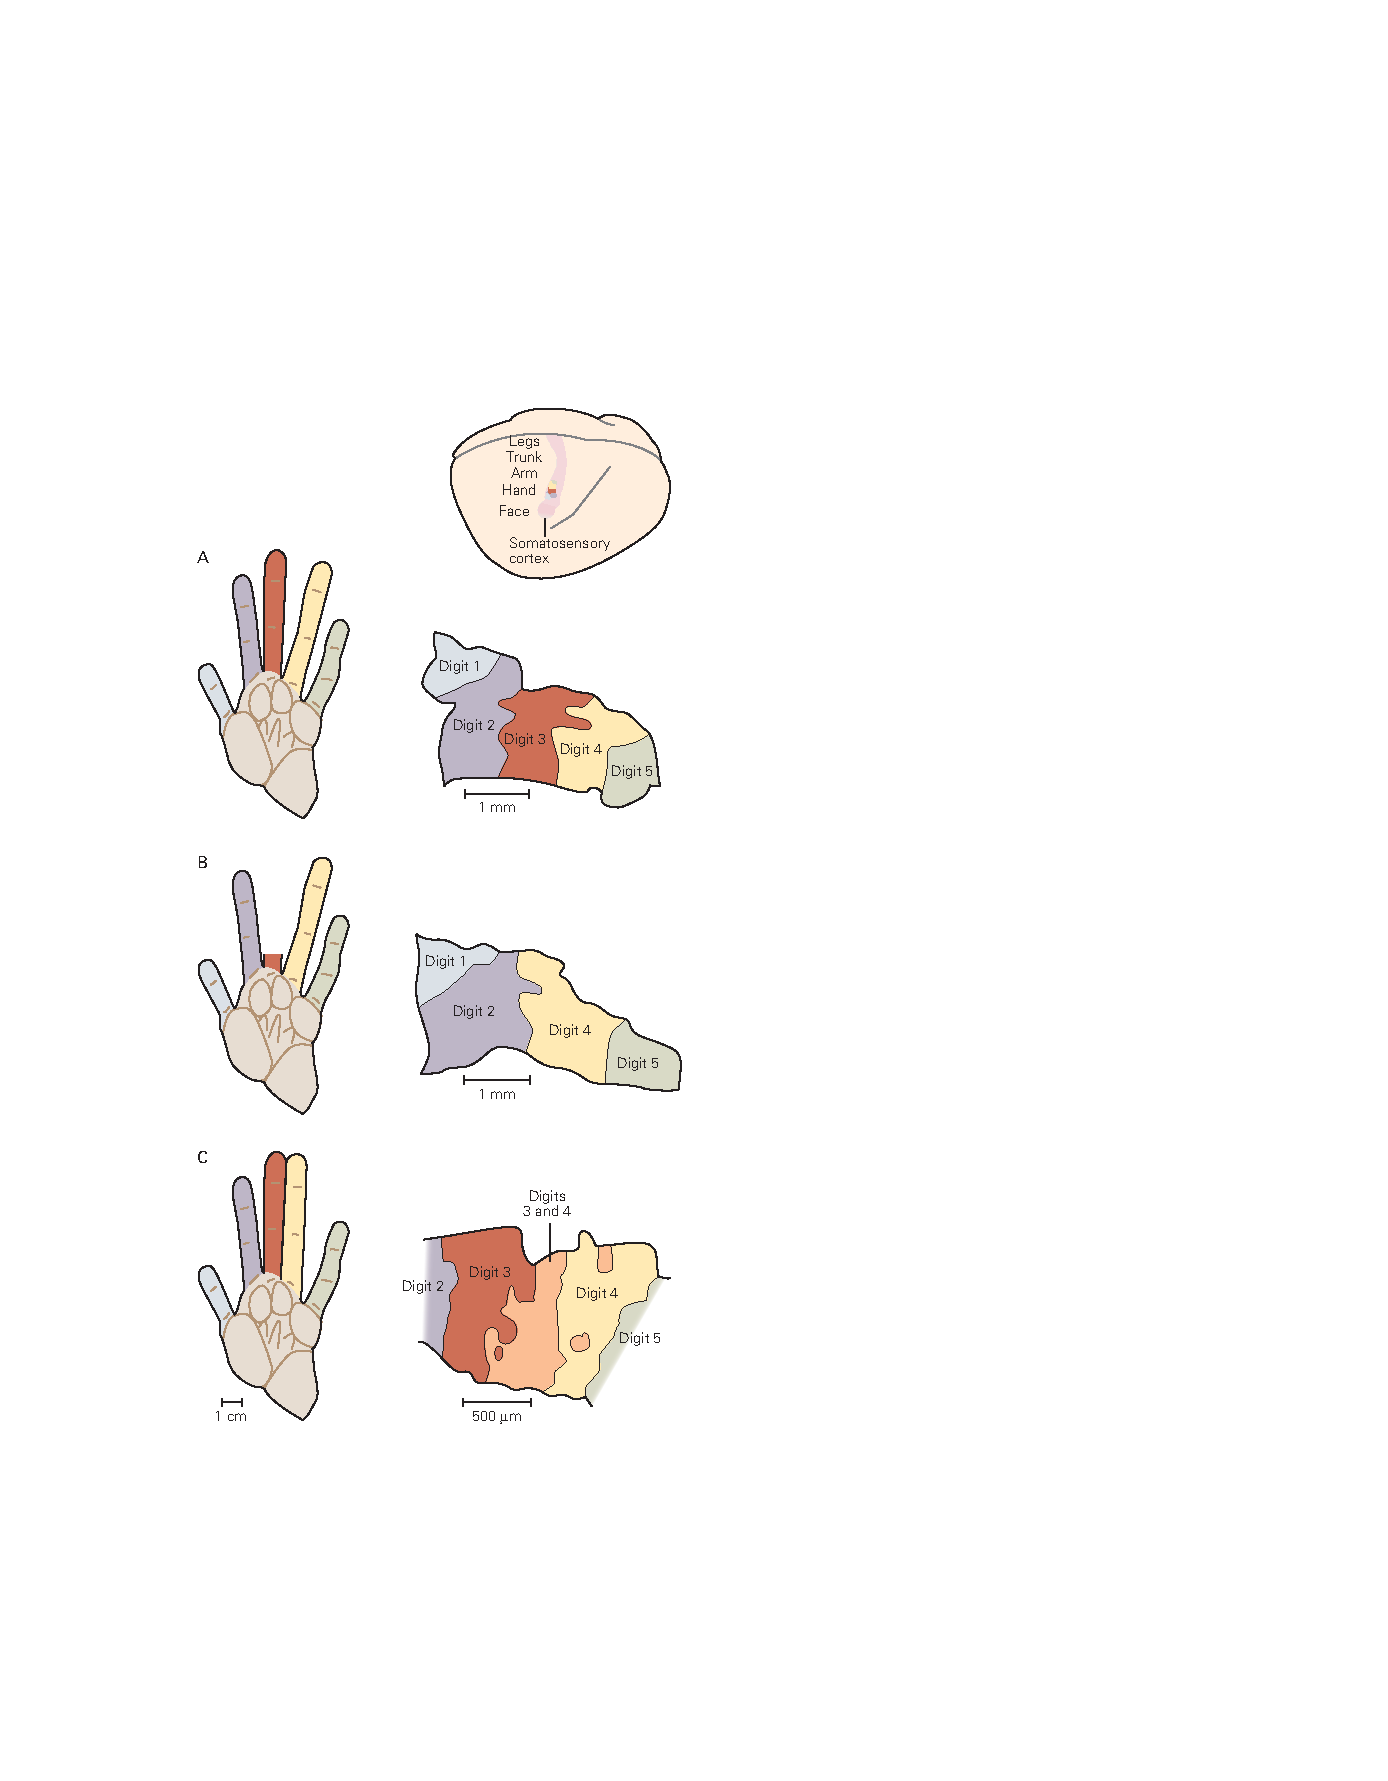
\includegraphics[width=0.68\linewidth]{chap49/fig_49_19}
	\caption{体感皮层中数字的表示可以在成年猴子中重新映射\cite{merzenich1984somatosensory}。
		\textbf{A.} 轻轻触摸手指上的特定点(左)会引起体感皮层神经元的反应(右),显示每个手指的有序地形图在皮层表面。
		突然的不连续性区分服务于相邻数字的区域。
		\textbf{B.} 截肢后,它先前提供的皮层区域没有反应。
		几个月后,相邻手指(2 和 4)的轴突在反应迟钝的区域形成了突触连接。
		\textbf{C.} 数字 3 和 4 缝合在一起后,它们同时受到感官刺激,代表数字的区域之间边界处的皮层区域对两者都有反应。}
	\label{fig:49_19}
\end{figure}


在\textit{梅策尼希}的研究之后的几年里,越来越多的证据表明,许多系统都可以重新开启关键时期。
我们通过返回两个关键时期已被很好地映射的区域来说明这一原则,即猫头鹰的视顶盖和小鼠的视觉皮层。



\subsection{视觉和听觉地图可以在成人中对齐}

在猫头鹰听觉和视觉地图匹配的初步研究中,用棱镜护目镜改变视野后的重新排列主要限于早期敏感期(图~\ref{fig:49_16}~和~\ref{fig:49_17})。
然而,三种策略显著增强了成年猫头鹰的双耳调谐可塑性。


\begin{figure}[htbp]
	\centering
	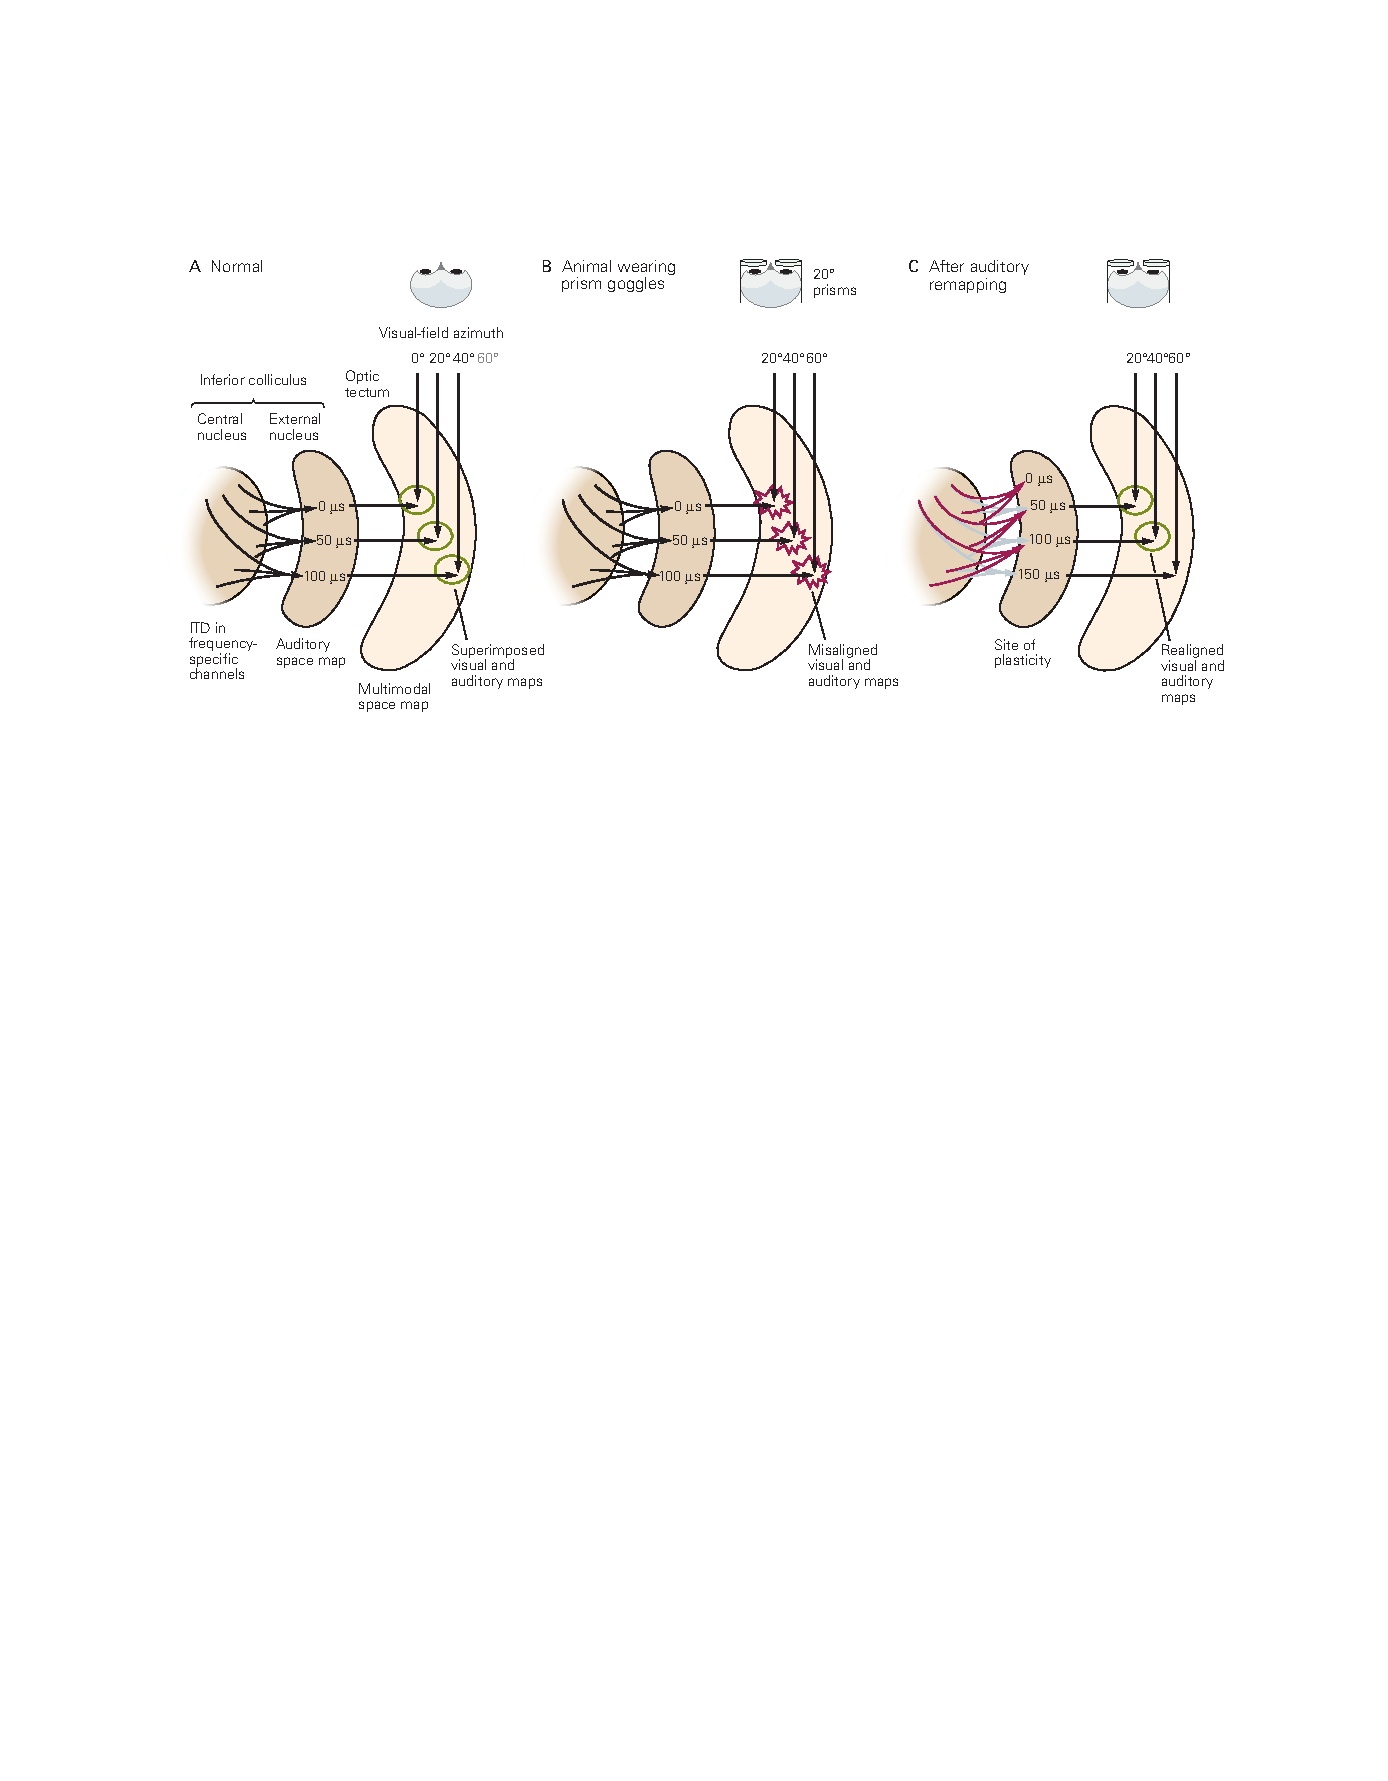
\includegraphics[width=1.0\linewidth]{chap49/fig_49_17}
	\caption{棱镜体验对仓鸮中脑听觉定位通路信息流的影响\cite{knudsen2002instructed}。
		\textbf{A.} 正常猫头鹰的听觉通路。
		\textit{双耳时间差}被测量并映射到脑干中特定频率的通道中。
		该信息上升到下丘,在那里创建了听觉空间的神经图。
		该地图被传送到视顶盖,在那里它与视觉空间的地图合并。
		\textbf{B.} 猫头鹰戴上棱镜护目镜后,视顶盖中的视觉和听觉空间映射变得错位。
		\textbf{C.} 重组听觉地图后,视觉和听觉地图再次对齐。}
	\label{fig:49_17}
\end{figure}


首先,当在青少年时期戴护目镜的成年猫头鹰重新戴上护目镜时,听觉地图再次移动以与新的视觉地图对齐(图~\ref{fig:49_20}A)。
相比之下,在青少年时期没有戴护目镜的成年猫头鹰中,护目镜的使用对听觉地图的组织几乎没有影响。
因此,正常关键时期的地图重排事件必须留下允许在以后的生活中重排的神经痕迹。
事实上,在生命早期佩戴棱镜的猫头鹰中,通常被修剪的听觉核的轴突得以保留,为成年后的重组提供了结构基础。


\begin{figure}[htbp]
	\centering
	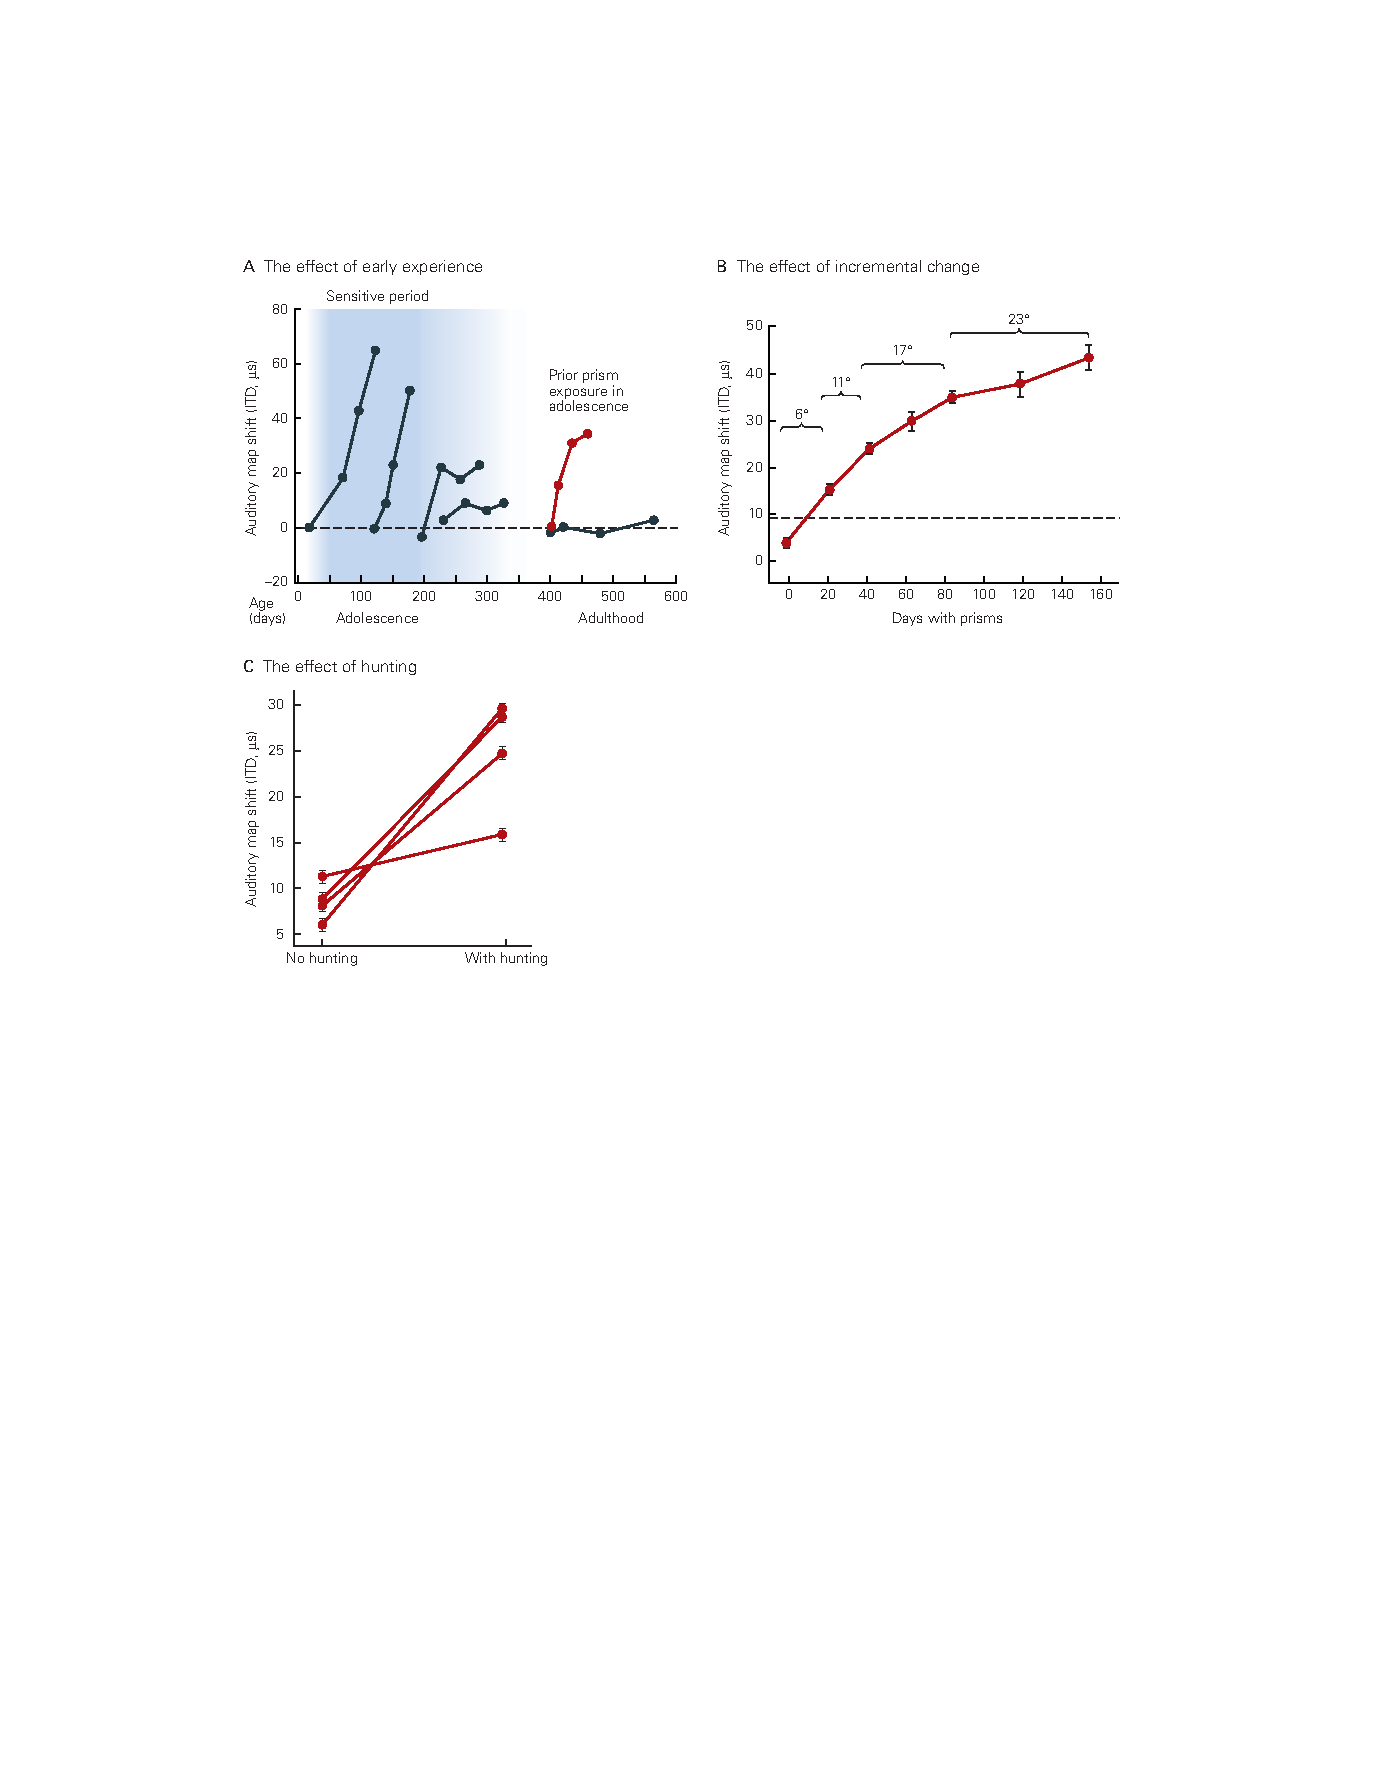
\includegraphics[width=1.0\linewidth]{chap49/fig_49_20}
	\caption{不同的行为条件对成年谷仓猫头鹰视觉和听觉神经图的重新排列有不同的影响。
		\textbf{A.} 在青春期短暂佩戴棱镜护目镜导致的听觉地图重塑留下了可以在成人中重新激活的神经痕迹。
		当这些鸟成年后戴上护目镜时,听觉地图仍然能够与视觉地图重新对齐。
		图像,听觉图已成功对齐。
		虚线表示如果动物在第 0 天安装了 23° 棱镜,则重新排列的范围。
		\textbf{C.} 如果一只成年猫头鹰有机会 戴着棱镜护目镜捕猎活的猎物时,会发生听觉重映射,这可能是因为增强了感知力的动机。}
	\label{fig:49_20}
\end{figure}


第二种诱导晚期可塑性的方法是让猫头鹰戴上一系列强度逐渐增加的棱镜眼镜,以小步移动视网膜图像。
在这些条件下,听觉图的调整通常比对单个大的视网膜图像位移的响应大三到四倍(图~\ref{fig:49_20}B)。


第三种技术是让猫头鹰捕食活的猎物。
在早期的实验中,动物是在标准实验室条件下饲养和饲养的。
然而,当佩戴棱镜的成年猫头鹰被允许在弱光条件下捕捉活老鼠 10 周时,它们表现出比喂食死老鼠的猫头鹰更大的双耳调谐可塑性(图~\ref{fig:49_19}C),尽管比幼年猫头鹰表现出的要小那没有打猎。
狩猎增加成年猫头鹰双耳调谐的可塑性这一发现戏剧性地证明了行为环境影响神经系统重组的能力。
这种影响是由增加的感官信息、注意力、唤醒、动机或奖励引起的,需要解决。



\subsection{双眼回路可以在成人中重塑}

随着对单眼剥夺的观察越来越多,很明显,一些可塑性在猫、大鼠和小鼠的经典关键期之后仍然存在。
例如,在小鼠中,即使一只眼睛在 2 或 3 个月大时被剥夺视力,眼优势也会发生适度的变化。
然而,到 4 个月大时,单眼剥夺没有可检测到的效果。


在过去的十年中,已经发现了几种干预措施可以增强年轻成年人的眼部优势可塑性程度,甚至可以使老年动物具有显著的可塑性。
有些是非侵入性的:环境丰富、社会互动(通过集体住房)、视觉刺激和锻炼都会增加成人单眼剥夺后发生变化的幅度和速度。
第二组干预措施针对的是似乎影响正常关键期时间的机制。
如上所述,用软骨素酶处理皮层以破坏神经元网或干扰髓磷脂对轴突生长的抑制作用可以延长和重新打开关键期。
值得注意的是,即使在 6 个月大的小鼠中,将未成熟的抑制性中间神经元移植到视觉皮层也会重新开启关键期。


我们如何调和关键时期的有力证据与成人回路重组的新证据?
与关键时期相比,在成人身上观察到的可塑性是适度和缓慢的,并且其机制在某些方面与早期剥夺的机制不同。
这些差异是由两个因素造成的。
首先,从出生后早期到青春期,大脑中的分子环境有利于轴突生长,细胞机制最适合促进突触的形成、加强、减弱和消除。
在这些条件下,回路很容易根据经验发生变化。
相反,在成熟的回路中,分子和结构元素促进稳定性并阻碍可塑性。
其次,在发展中的回路中,没有任何特定的连接模式是牢固确立的,因此需要克服的东西更少。
由遗传决定因素指定的联系不太精确,而且联系本身也相对较弱。
经验产生的神经活动模式会强化甚至重新调整这些连接模式。


总而言之,关键时期的经验对回路具有强大的影响,因为细胞和分子条件对于可塑性是最佳的,并且因为指导的连接模式不必与长期存在的模式竞争。
这些差异有助于解释刺激成人可塑性所需的特殊行为、药理学或遗传干预。



\section{要点}

1. 尽管神经系统在整个生命过程中都具有可塑性,但可塑性在出生后早期生命的有限时间间隔内(称为关键期)特别大。
在这些时期发生的变化几乎是不可逆转的。


2. 关键时期因大脑区域和任务而异。
例如,患有斜视(斜眼)的儿童永远不会有良好的立体视觉,除非他们的眼睛在出生后的最初几年内调整好,而且人们在十几岁后就无法学习一门没有口音的新语言。


3. 对关键时期最丰富的理解来自\textit{休伯尔}和\textit{威泽尔}发起的关于双眼输入如何整合到皮层的研究。
他们在幼猫或猴子的不同时期剥夺了一只眼睛的视力。
在正常动物中,视觉皮层中的大多数神经元都对双眼有反应,但在出生后早期短暂的单眼剥夺后,大多数皮层细胞会永久失去对来自曾经闭上的眼睛的输入的反应。
眼睛本身和外侧膝状体的反应几乎正常,将皮层定位为变化部位。
成年后更长时间的剥夺几乎没有影响。


4. 在眼优势列的交替模式中可以看到双眼功能丧失的结构基础,其中神经元由一只眼睛或另一只眼睛的输入支配。
在关键时期单眼剥夺之后,代表睁眼的柱子以代表闭眼的柱子为代价扩大了。
这种形式的可塑性可能旨在优化每个人在每个时间段对皮层空间的使用,例如,随着头部的长大和眼睛变得更远,双眼相互作用会发生微妙的变化。


5. 双眼相互作用反映了两组输入之间的竞争,因为在双眼剥夺后视觉和对称柱被保留。
许多证据表明,竞争取决于两只眼睛中出现的活动模式,每只眼睛的输入比另一只眼睛的输入更同步。
出生后,同步是由视觉体验驱动的。
产前或睁眼之前,两只眼睛的模式化自发活动是同步的原因。


6. 单眼剥夺效应背后的细胞机制已在小鼠身上进行了最详细的研究。
在单眼剥夺之后,来自闭眼的输入通过类似于\textit{长时程抑制}的过程迅速减弱。
此后不久,另一只眼睛的输入得到加强,部分原因是一种称为稳态可塑性的补偿机制。
丘脑轴突和皮层树突的结构重塑发生较晚。


7. 抑制性中间神经元的成熟是关键期何时开启的主要决定因素。
关键期结束的标志是髓鞘和富含蛋白聚糖的神经元周围结构的形成,这些结构阻碍了结构重塑。


8. 虽然双眼相互作用的可塑性最初被认为仅限于出生后早期,但现在很明显,成人的关键时期可以在某种程度上“重新开启”。
在某些情况下,这可以通过改变动物的环境或改变体验的传递方式来实现。
关键期也可以通过操纵一些通常在青春期关闭它们的因素来重新打开。


9. 与产后早期关键期相比,成年期的可塑性程度适中且难以触发。
尽管如此,如果控制得当,关键时期的重新开放可以使重组能够弥补因受伤、疾病和早期适应不良经历造成的损失。


10. 关键时期出现在许多系统的发展过程中,例如形成有序的听觉、体感和视觉输入到相关感觉皮层的映射。
许多表征双眼交互可塑性的原理和机制也调节这些关键时期,包括自发和依赖经验的活动、竞争、兴奋性和抑制性突触的改变以及输入的选择性增长和修剪以实现适当模式的作用。 成人连接。


11. 关键期的存在表明大脑的重塑能力在成年期急剧下降。
这似乎是不利的,但可能代表一种有用的适应,允许每个大脑在其发育过程中适应其环境,然后缓冲它以防止以后的过度变化,甚至可能使技能和记忆持续存在。
如果是这种情况,基于重新开启成人关键期的疗法可能会付出代价。



